%!TEX TS-program = xelatex

\documentclass[t]{beamer}  % [t], [c], или [b] --- вертикальное выравнивание на слайдах (верх, центр, низ)
%\documentclass[t, handout]{beamer} % Раздаточный материал (на слайдах всё сразу)
%\documentclass[aspectratio=169, t]{beamer} % Соотношение сторон

\usepackage{epstopdf}

%\usetheme{Berkeley} % Тема оформления
%\usetheme{Bergen}
%\usetheme{Szeged}

%\usecolortheme{beaver} % Цветовая схема
%\useinnertheme{circles}
%\useinnertheme{rectangles}

\usepackage{HSE-theme/beamerthemeHSE} % Подгружаем тему


%%% Работа с русским языком
\usepackage{cmap}					% поиск в PDF
\usepackage{mathtext} 				% русские буквы в формулах
\usepackage[T2A]{fontenc}			% кодировка
\usepackage[utf8]{inputenc}			% кодировка исходного текста
%%% Работа с русским языком и шрифтами
\usepackage[english,russian]{babel}   % загружает пакет многоязыковой вёрстки


%%% Дополнительная работа с математикой
\usepackage{amsmath,amsfonts,amssymb,amsthm,mathtools} % AMS
\usepackage{icomma} % "Умная" запятая: $0,2$ --- число, $0, 2$ --- перечисление

%% Номера формул
%\mathtoolsset{showonlyrefs=true} % Показывать номера только у тех формул, на которые есть \eqref{} в тексте.
%\usepackage{leqno} % Нумерация формул слева

%% Свои команды
\DeclareMathOperator{\sgn}{\mathop{sgn}}

%% Перенос знаков в формулах (по Львовскому)
\newcommand*{\hm}[1]{#1\nobreak\discretionary{}
	{\hbox{$\mathsurround=0pt #1$}}{}}

%%% Работа с картинками
\usepackage{graphicx}  % Для вставки рисунков
\graphicspath{{images/}{images2/}}  % папки с картинками
\setlength\fboxsep{3pt} % Отступ рамки \fbox{} от рисунка
\setlength\fboxrule{1pt} % Толщина линий рамки \fbox{}
\usepackage{wrapfig} % Обтекание рисунков текстом
\usepackage{caption}


%%% Работа с таблицами
\usepackage{array,tabularx,tabulary,booktabs} % Дополнительная работа с таблицами
\usepackage{longtable}  % Длинные таблицы
\usepackage{multirow} % Слияние строк в таблице

%%% Программирование
\usepackage{etoolbox} % логические операторы

%%% Другие пакеты
\usepackage{lastpage} % Узнать, сколько всего страниц в документе.
\usepackage{soul} % Модификаторы начертания
\usepackage{csquotes} % Еще инструменты для ссылок
%\usepackage[style=authoryear,maxcitenames=2,backend=biber,sorting=nty]{biblatex}
\usepackage{multicol} % Несколько колонок

%%% Картинки
\usepackage{tikz} % Работа с графикой
\usepackage{pgfplots}
\usepackage{pgfplotstable}
\usepackage{verbatim}
\usetikzlibrary{fadings}
\usepackage[outline]{contour}
\usepackage{pifont} 
\usepackage{adjustbox}

\usepackage{chngcntr} % нумерация графиков и таблиц по секциям
\counterwithin{table}{section}
\counterwithin{figure}{section}

\usepackage{listings}

\lstdefinelanguage{Rust}{
  sensitive=true,
  morekeywords=[1]{
    break, continue, else, for, if, loop, match, return, while, struct
  },
  morekeywords=[2]{
    crate, fn, async, mod, pub, use, self, Self, struct, enum, const, static, let, mut, ref, type, impl, trait, where, as, dyn, move,
  },
  morekeywords=[3]{
    bool, char, i8, i16, i32, i64, isize, u8, u16, u32, u64, usize, f32, f64, str, String,
  },
  morekeywords=[4]{
    Ok, Err, Some, None,
  },
  morekeywords=[5]{
    await,
  },
  keywordstyle=[5]{\color{purple}},
  morecomment=[s]{/*}{*/},
  morecomment=[l]//,
  morestring=[b]",
  morestring=[b]r",
  morestring=[b]'',
}

\lstset{
  language=Rust,
  basicstyle=\ttfamily,
  keywordstyle=\color{blue},
  stringstyle=\color{red},
  commentstyle=\color{green},
  showstringspaces=false,
  breaklines=true,
  frame=none,
}


\lstnewenvironment{rustcode}[1][]{
  \lstset{
    language=Rust,
    basicstyle=\ttfamily,
    keywordstyle=\color{blue},
    stringstyle=\color{red},
    commentstyle=\color{gray},
    showstringspaces=false,
    breaklines=true,
    % frame=single,
    #1
  }
}{}


\lstnewenvironment{cppcode}[1][]{
  \lstset{
    language=C++,
    basicstyle=\ttfamily,
    keywordstyle=\color{blue},
    stringstyle=\color{red},
    commentstyle=\color{gray},
    showstringspaces=false,
    breaklines=true,
    % frame=single,
    #1
  }
}{}

\usepackage{setspace}
\usepackage{color}



\title{Разработка симулятора вычислительного кластера}
\author[Артём Макогон]{\footnotesize Выполнил: Макогон Артём Аркадьевич, БПМИ206 \\[5pt]   Руководитель: Сухорослов Олег Викторович, к.т.н, доцент НИУ ВШЭ}
\date{\today}
% \institute[Высшая школа экономики]{National Research University\\ 
	% <<Higher School of Economics>>}



\begin{document}
	
	\begin{frame}
		\maketitle
	\end{frame}
	
    \section{Введение}
    \subsection{Описание предметной области}

	\begin{frame}[fragile]
		\frametitle{\insertsection} 
		\framesubtitle{\insertsubsection}
				\vspace{0.5cm}
				\begin{itemize}
					\item Вычислительные кластеры активно используются в исследованиях и компаниях.
					\item От качества алгоритма планирования задач зависит эффективность использования ресурсов.
					\item При разработке алгоритмов их необходимо тестировать.
				\end{itemize}
				\alt<2->{
					{ \hspace{5cm} \large $\Downarrow$ } 
					\begin{itemize}
						\item[\small\textgreater] Использовать реальный кластер долго и дорого.
						\item[\small\textgreater] Необходимо обеспечивать воспроизводимость результатов.
					\end{itemize}
				}{}
				\alt<3->{
					{ \hspace{5cm} \large $\Downarrow$ } 
					\begin{itemize}
						\item[\small\ding{51}] Используются \textbf{симуляторы}.
					\end{itemize}
				}{}
		
	\end{frame}

	\subsection{Архитектура кластера}

	\begin{frame}[fragile]
    \frametitle{\insertsection} 
	\framesubtitle{\insertsubsection}
	\vspace{0.1cm}	
	\begin{figure}[H]
		\centering
			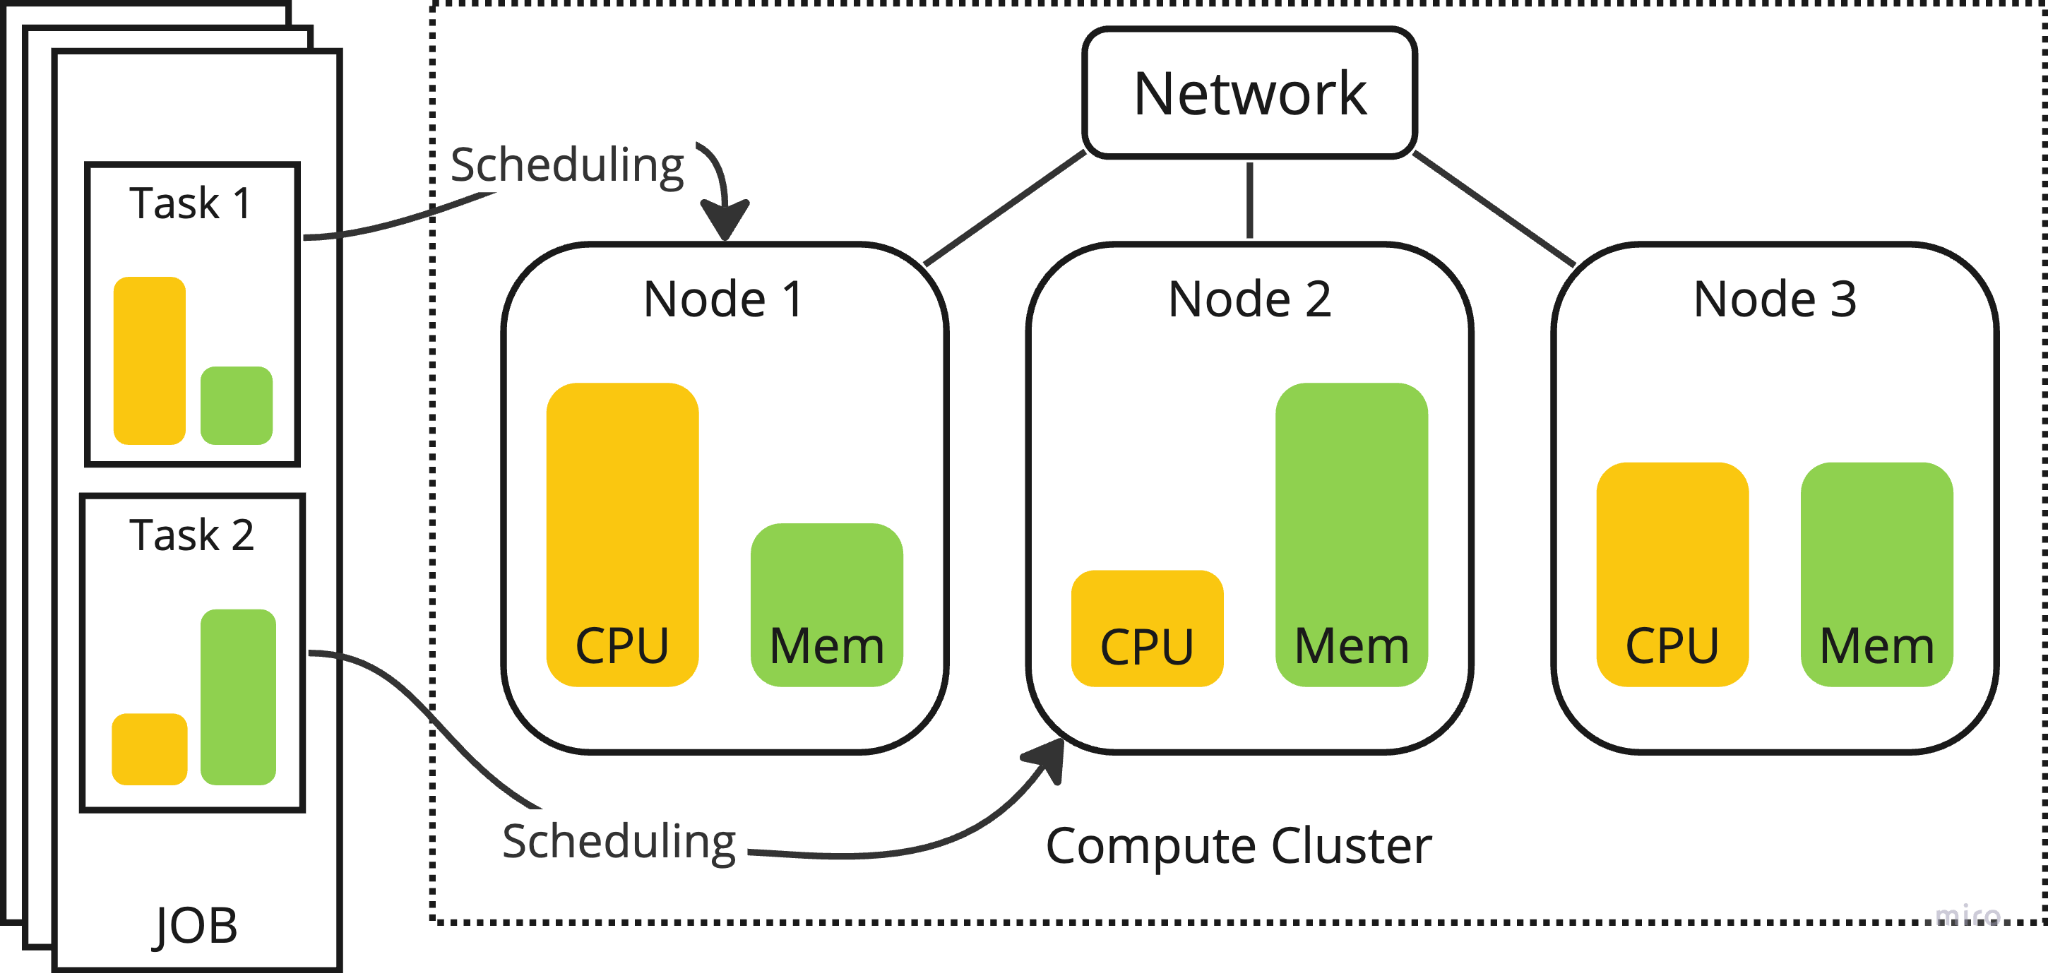
\includegraphics[width=\linewidth]{images/cluster_network}
			\vspace{0.1cm}
			\caption*{Модель архитектуры кластера}
		\end{figure}


	\end{frame}

	\subsection{Симуляция кластера}

	\begin{frame}[fragile]
		\frametitle{\insertsection} 
		\framesubtitle{\insertsubsection}
		\vspace{0.1cm}	
		\begin{figure}[H]
			\centering
				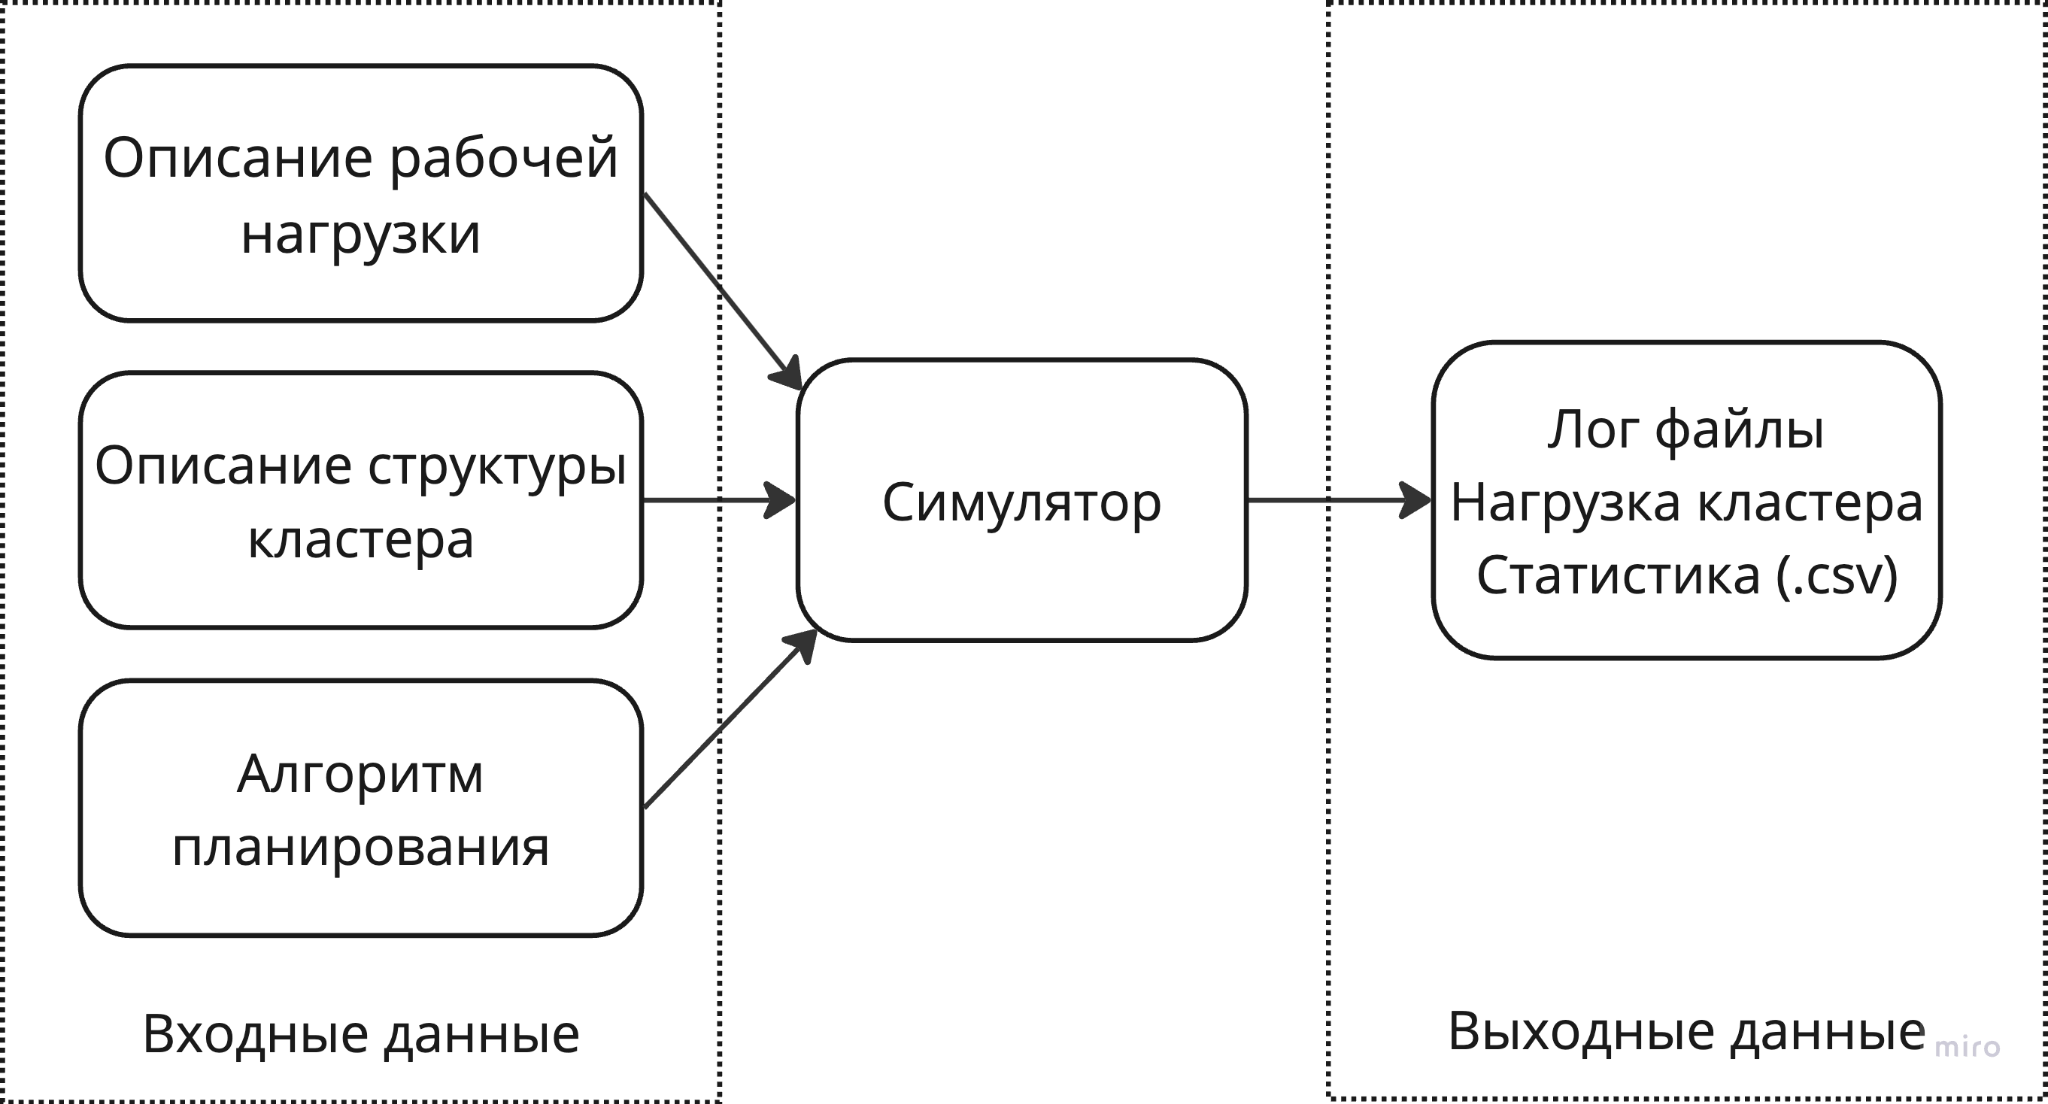
\includegraphics[width=\linewidth]{images/input_output_data}
				\vspace{0.1cm}
				\caption*{Входные и выходные данные симулятора}
			\end{figure}
	
	
		\end{frame}


	\subsection{Модель рабочей нагрузки на кластер}


	\begin{frame}[fragile]
		\frametitle{\insertsection} 
		\framesubtitle{\insertsubsection}
		\vspace{0.5cm}
		Рабочая нагрузка состоит из заданий (job), которые делятся на задачи (tasks). 

		\alt<2->{
		\vspace{0.5cm}
		Структуры заданий: 
		\begin{itemize}
			\item \texttt{rigid} -- фиксированные требования к ресурсам
			\item \texttt{moldable} -- адаптивные требования к ресурсам 
			\item \texttt{malleable} -- гибкие требование к ресурсам
		\end{itemize}
		}{}
		
		\alt<3->{
		\vspace{0.5cm}
		Требования к планированию: 

		\begin{itemize}
			\item Раздельное планирование (MapReduce)
			\item Комплектное планирование (Gang Scheduling, Slurm)
		\end{itemize}
		}{}
	\end{frame}

	\subsection{Виды входных данных для симулятора}

    \begin{frame}[fragile]
    \frametitle{\insertsection} 
	\framesubtitle{\insertsubsection}
	
			\vspace{0.5cm}
	\begin{columns}[t]
		\begin{column}{0.55\textwidth}
			{\centering \small\texttt{Standard Workload Format (SWF)}}
			\vspace{0.3cm}
			\begin{itemize}
				\item<1-> CPU/RAM 
				\item<2-> Дано время исполнения и требования к ресурсам
				\item<2-> Нагрузка вычисляется тривиально
				\item<3-> Используется в популярных трейсах (Google, Alibaba, и т.д.)
			\end{itemize}
						
		\end{column}
		\begin{column}{0.5\textwidth}
			{\centering  \small\texttt{Custom workloads}}
			\vspace{0.3cm}
			\begin{itemize}
				\item<1-> CPU/RAM/disk/network 
				\item<2-> Дана нагрузка и ресурсы
				\item<2-> Время вычисляется с помощью моделей
				\item<3-> Обычно NDA
			\end{itemize}
		\end{column}
	\end{columns}


    \end{frame}




	

	 
	\subsection{Постановка задачи}
	\begin{frame}[fragile]
		\frametitle{\insertsection} 
		\framesubtitle{\insertsubsection}
		\vspace{0.5cm}
		\underline{Цель проекта} -- разработать симулятор вычислительного кластера на базе фреймворка DSLab. Для этого необходимо:
		\begin{itemize}
			\item Изучить литературу по теме и существующие симуляторы, подготовить обзор с анализом
			их преимуществ и недостатков.
			\item Реализовать компоненты симулятора.
			\item Написать документацию и тесты.
			\item Подготовить и провести эксперименты, демонстрирующие работоспособность симулятора.
		\end{itemize}
	\end{frame}






	\section{Обзор литературы}
	\subsection{Существующие симуляторы}
	\begin{frame}
		\frametitle{\insertsection} 
		\framesubtitle{\insertsubsection}

		\begin{figure}[H]
			\hspace{-1.1cm}
			\centering
			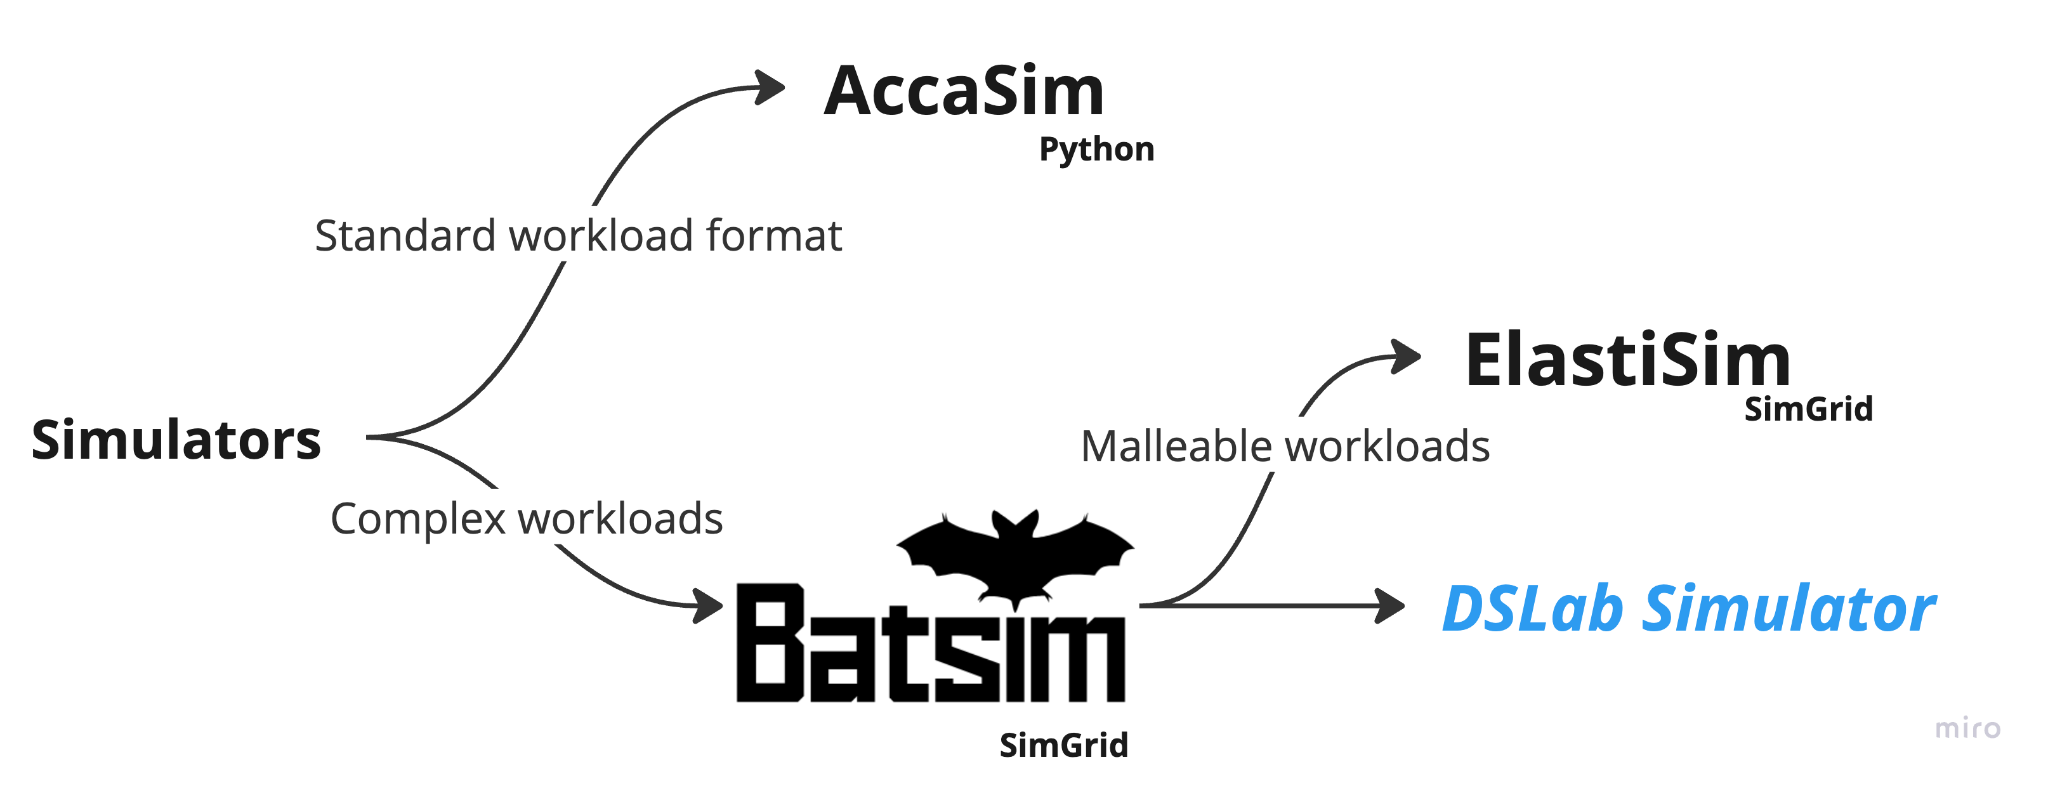
\includegraphics[width=1.1\linewidth]{images/simulators}
			\vspace{0.2cm}
			\caption*{Существующие симуляторы}
		\end{figure}
	\end{frame}






	\section{Реализация симулятора}

	\subsection{Архитектура DSLab}
	\begin{frame}[fragile]
		\frametitle{\insertsection} 
		\framesubtitle{\insertsubsection}
		\vspace{0.5cm}
		\begin{figure}[H]
			\centering
			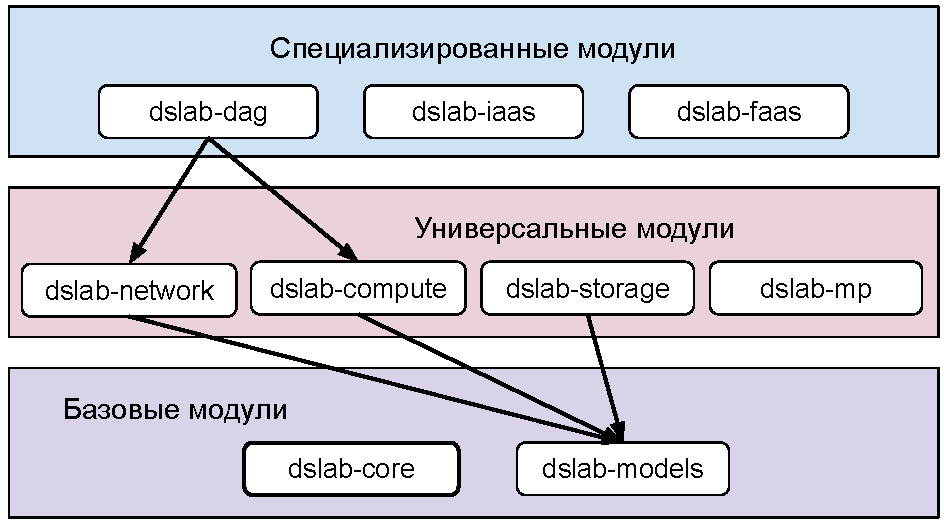
\includegraphics[width=\linewidth]{images/dslab_arc}
			\caption*{Архитектура фреймворка DSLab}
		\end{figure}
	\end{frame}


	\subsection{Асинхронное управление событиями. Комбинаторы \texttt{futures}}


	\begin{frame}[fragile]
		\frametitle{\insertsection} 
		\framesubtitle{\insertsubsection}
		\begin{columns}[t]
			\begin{column}{0.6\linewidth}
			\begin{figure}
				\centering
				\scriptsize

				\begin{rustcode}
async fn process_task(&self, req: TaskRequest) {
  let mut task = TaskInfo {req};

  self.download_data(&task).await;
  self.read_data(&task).await;
  self.run_task(&task).await;
  self.write_data(&task).await;
  self.upload_result(&task).await;
}
				\end{rustcode}

				\caption*{Пример последовательных задач.}

			\end{figure}
		\end{column}

		\begin{column}{0.6\linewidth}
\begin{figure}[H]
    \scriptsize
\begin{rustcode}
async fn run(&self, args: JobArgs){    
  futures::join!(
    self.download_data(args.node_1),
    self.download_data(args.node_2),       
  )
}
\end{rustcode}
\vspace{1.3cm}
\caption*{Пример параллельных задач.}
\end{figure}	
		\end{column}
		\end{columns}
	\end{frame}





	\subsection{Архитектура симулятора}

	\begin{frame}[fragile]
		\frametitle{\insertsection} 
		\framesubtitle{\insertsubsection}
		
		\vspace{0.5cm}
\begin{figure}[H]
	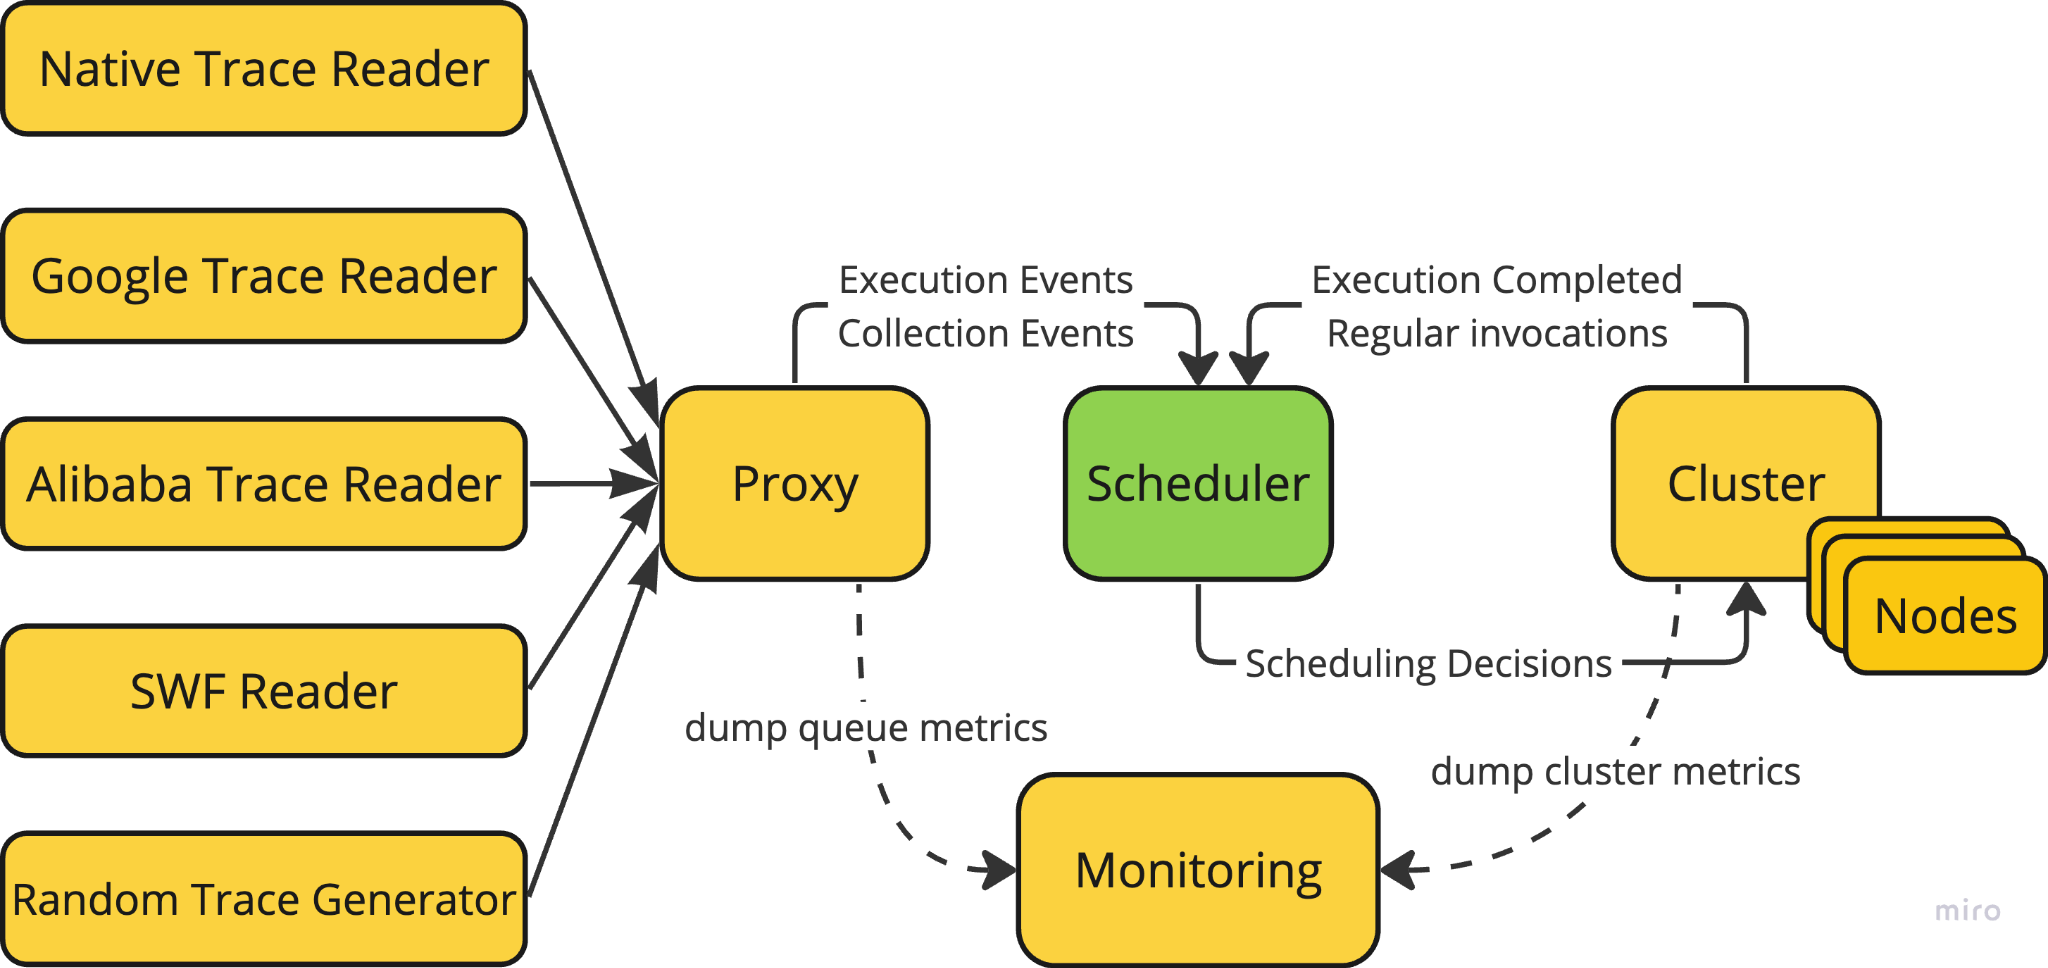
\includegraphics[width=\linewidth]{images/cluster-design-colored}
	% 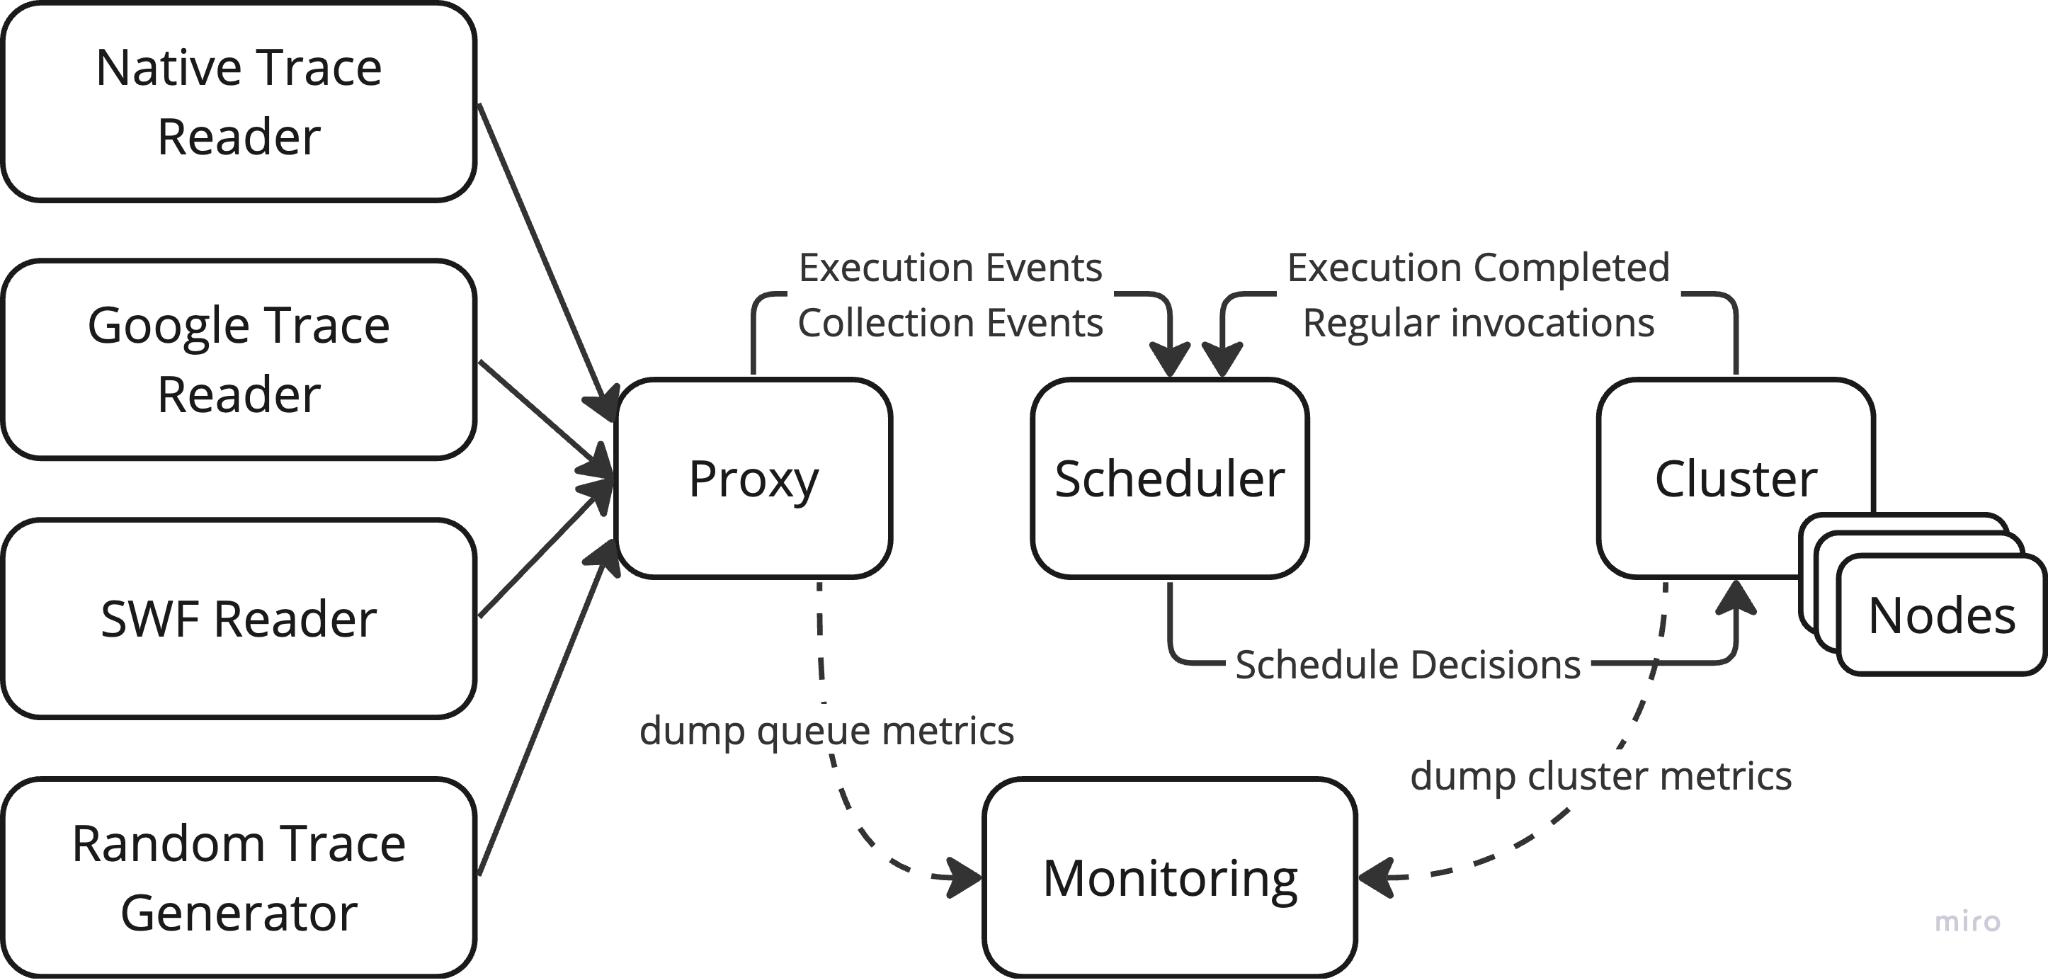
\includegraphics[width=\linewidth]{images/simulator_arc}
	\vspace{0.2cm}
	\caption*{Архитектура симулятора}
\end{figure}

	\end{frame}


	\subsection{Модель кластера}

	\begin{frame}[fragile]
		\frametitle{\insertsection} 
		\framesubtitle{\insertsubsection}


		\vspace{1.5cm}
\begin{table}[H]
	\footnotesize
    \centering
    \begin{tabular}{|l|l|c|}
    \hline
    \textbf{Название модуля} & \textbf{Используемый модуль} & \textbf{Обязательный} \\
    \hline
    \texttt{compute} & \texttt{dslab\_compute::multicore::Compute} & да \\
    \hline
    \texttt{network} & \texttt{dslab\_network::Network} & нет  \\
    \hline
    \texttt{disk} & \texttt{dslab\_storage::disk::Disk} & нет \\
    \hline
    \end{tabular}
    \caption*{Модули каждого сервера в кластере}
    \label{tab:server_modules}
\end{table}
\end{frame}


\subsection{Модель сети \texttt{Fat-Tree-Topology}}
\begin{frame}[fragile]
	\frametitle{\insertsection}
	\framesubtitle{\insertsubsection}

\begin{figure}[H]
	\centering 
	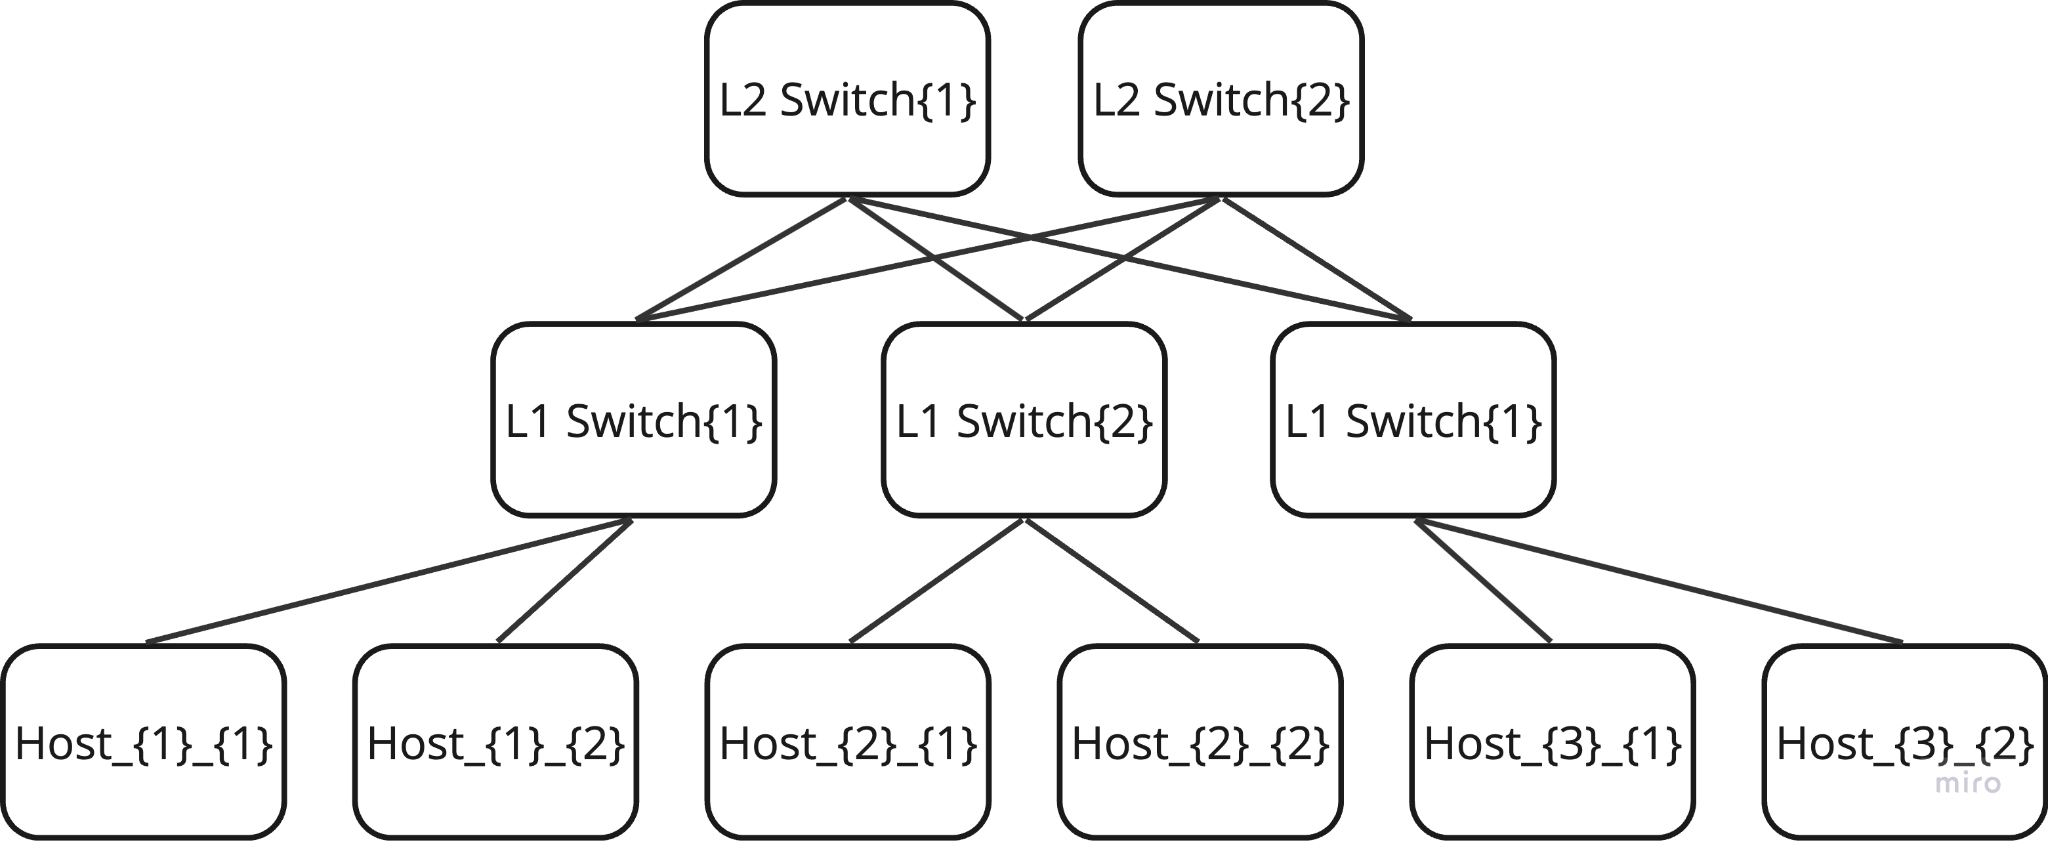
\includegraphics[width=\linewidth]{images/fat_tree_topology}
	\vspace{0.2cm}
	\caption*{Модель сети \texttt{Fat-Tree-Topology} в кластере}
\end{figure}
	\end{frame}

	\subsection{Деление на \texttt{Collection} и \texttt{Execution}}


	\begin{frame}[fragile]
		\frametitle{\insertsection} 
		\framesubtitle{\insertsubsection}

		\begin{table}[H]
			\scriptsize
			\centering
			\begin{tabular}{|l|l|p{7cm}|}
				\hline
				\textbf{Поле} & \textbf{Тип} & \textbf{Описание} \\ 
				\hline
				id & \texttt{u64} & Уникальный идентификатор задания \\
				\hline
				user & \texttt{Option<String>} & Пользователь, который запускает задание.  \\
				\hline
				priority & \texttt{Option<u64>} & Приоритет задания. \\
				\hline
				... & ... & ... \\
				\hline
			\end{tabular}
			\caption*{Описание структуры данных \texttt{Collection}}
			\label{tab:collection}
		\end{table}

\vspace{-0.5cm}

\begin{table}[h]
    \centering
	\scriptsize
    \begin{tabular}{|l|l|p{5cm}|}
        \hline
        \textbf{Поле} & \textbf{Тип} & \textbf{Описание} \\
        \hline
        id & \texttt{u64} & Уникальный идентификатор задачи \\
        \hline
        collection\_id & \texttt{Option<u64>} & Индекс задания  \\
        \hline
        time & \texttt{f64} & Время, когда задача становится доступной для планирования \\
		\hline
        resources & \texttt{ResourceRequirements} & Структура требуемых ресурсов \\
        \hline
        profile & \texttt{Rc<dyn ExecutionProfile>} & Профиль нагрузки \\
        \hline
		... & ... & ... \\
		\hline
    \end{tabular}
    \caption*{Описание структуры данных \texttt{Execution}}
\end{table}

	\end{frame}


	\subsection{Модель планировщика}
\begin{frame}[fragile]
	\frametitle{\insertsection} 
	\framesubtitle{\insertsubsection}
	\vspace{-1cm}
	\begin{columns}
		\begin{column}{1.1\linewidth}
	\begin{figure}[H]
		\fontsize{7.5}{10}\selectfont
		\begin{rustcode}
pub trait Scheduler {
  fn on_host_added(&mut self, ctx: &Context, host: HostConfig);
  fn on_execution_request(&mut self, ctx: &Context, req: Execution);
  fn on_collection_request(&mut self, ctx: &Context, req: Collection);
  fn on_execution_finished(&mut self, ctx: &Context, execution_id: u64);
  fn on_host_notification(&mut self, ctx: &Context, host_id: Id, resources: ResourcesPack);
}
		\end{rustcode}
		\vspace{-0.5cm}
		\caption*{Интерфейс планировщика \texttt{Scheduler}}
	\end{figure}

\end{column}
\end{columns}

% \vspace{-0.5cm}

\begin{columns}
	\begin{column}{1.1\linewidth}
{
	\small
	\begin{itemize}
\item<2-> Возможности контекста: 
	\begin{enumerate}
		\item Запланировать/отменить задачу (полная отмена недоступна) 
		\item<3-> Доступ к генератору случайных чисел симуляции
	\end{enumerate}
\item<4-> Можно реализовать планировщик как компонент симуляции и получить больше возможностей (например, асинхронность).
\end{itemize}
}
\end{column}
\end{columns}

\end{frame}


\subsection{Trait ExecutionProfile}

	\begin{frame}[fragile]
		\frametitle{\insertsection} 
		\framesubtitle{\insertsubsection}
		
\begin{figure}[H]
	\centering
	\hspace*{-0.5cm}
	\begin{minipage}{1.15\linewidth}
    \scriptsize
\begin{rustcode}
#[async_trait(?Send)]
pub trait ExecutionProfile {
  async fn run(self: Rc<Self>, processes: &Vec<HostProcessInstance>);
}
\end{rustcode}
	\end{minipage}
\caption*{Интерфейс \texttt{ExecutionProfile}}
\end{figure}

\vspace{-1cm}

\begin{figure}[H]
	\centering
	\hspace*{-0.6cm}
	% 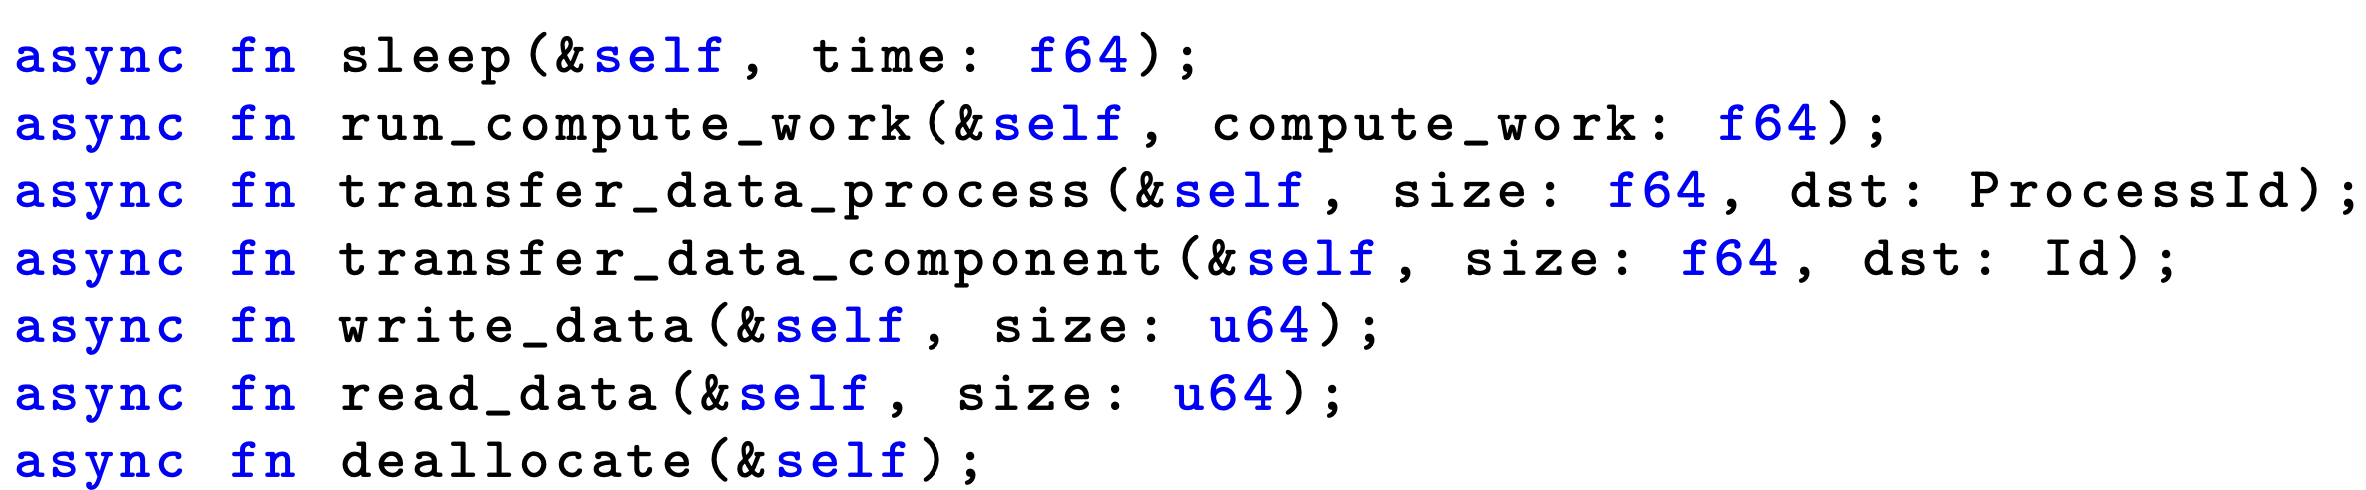
\includegraphics[width=\linewidth]{images/profile_interface}
	\begin{minipage}{1.15\linewidth}
    \scriptsize
\begin{rustcode}
async fn sleep(&self, time: f64);
async fn run_compute_work(&self, compute_work: f64);
async fn transfer_data_process(&self, size: f64, dst: ProcessId);
async fn transfer_data_component(&self, size: f64, dst: Id);
async fn write_data(&self, size: u64);
async fn read_data(&self, size: u64);
async fn deallocate(&self);
\end{rustcode}
\end{minipage}
\caption*{Интерфейс взаимодействия процессов с кластером}
\end{figure}



	\end{frame}


	\subsection{Пример реализации \texttt{ExecutionProfile}}

\begin{frame}[fragile]
	\frametitle{\insertsection} 
	\framesubtitle{\insertsubsection}

\vspace{0.2cm}

\begin{figure}
	\centering 
	\includegraphics<1>[width=\linewidth]{images/mw_code_1}
	\includegraphics<2>[width=\linewidth]{images/mw_code_2}
	\includegraphics<3>[width=\linewidth]{images/mw_code_3}
	\includegraphics<4>[width=\linewidth]{images/mw_code_4}
\end{figure}
% \begin{columns}
% 	\begin{column}{1.1\linewidth}
% 	\hspace*{-0.1cm}
% 	\fontsize{7.5}{8}\selectfont
% 	\begin{rustcode}
% pub struct MasterWorkersProfile {
%   pub master_compute_work: f64,
%   pub worker_compute_work: f64,
%   pub data_transfer_size: f64,
% }
% 	\end{rustcode}

% 	\begin{rustcode}
% #[async_trait(?Send)]
% impl ExecutionProfile for MasterWorkersProfile {
%   async fn run(self: Rc<Self>, processes: &Vec<HostProcessInstance>) {
%     let master = &processes[0];
%     let workers = &processes[1..];
% 	\end{rustcode}
% 	\begin{rustcode}
%     futures::future::join_all(workers.iter().map(|p| async {
%       master.transfer_data_process(self.data_transfer_size, p.id).await;
%       p.run_compute(self.worker_compute_work).await;
%     }))
%     .await;
    
%     master.run_compute(self.master_compute_work).await;
%   }
% }
% 		\end{rustcode}

% 	\end{column}
% \end{columns}

\end{frame}

\subsection{Пример описания рабочей нагрузки через файл \texttt{YAML}}

\begin{frame}[fragile]
	\frametitle{\insertsection}
	\framesubtitle{\insertsubsection}

	\vspace{-1cm}
	\begin{columns}
		\scriptsize
	\begin{column}{0.5\textwidth}
		\begin{figure}[H]
			\centering
		\begin{yamlcode}
compute-simple: 
  type: compute-homogenous
  args: 
	compute_work: 1000.0 
compute-hard:
  type: compute-homogenous
  args:
	compute_work: 2000.0
net-all-to-all-simple:
  type: communication-homogenous
  args: 
	size: 500.0 
disk-simple-read: 
  type: disk-read 
  args: 
	size: 1000
		\end{yamlcode}
		\caption*{Пример описания базовых профилей}
	\end{figure}
	\end{column}
	\hspace{-0.5cm}
	\begin{column}{0.6\textwidth}
		\begin{figure}[H]
			\centering
		\begin{yamlcode}
complex_execution_profile:
  type: sequence
  args:
    repeat: 2
    profiles:
      - disk-simple-read
      - compute-simple
      - parallel
    	args:
    	  profiles:
            - compute-hard
            - net-all-to-all-simple
      - disk-simple-write-part
      - parallel
    	args:
    	  profiles:
            - compute-simple
            - net-all-to-all-simple
      - disk-simple-write-part
	\end{yamlcode}
	\vspace{-0.2cm}
		\caption*{Пример описания профиля через комбинаторы}
\end{figure}
	\end{column}
	\end{columns}

\end{frame}


\section{Сравнение с \texttt{BatSim}}
\subsection{Модель рабочей нагрузки}

\begin{frame}[fragile]
	\frametitle{\insertsection} 
	\framesubtitle{\insertsubsection}
	\vspace{-0.5cm}
	\begin{figure}
		\scriptsize
	\begin{jsoncode}
"jobs": [
  {"id": "job1",  ...  "res": 4, "profile": "sequence"},
],

"profiles": {
  "homogeneous": {
    "type": "parallel_homogeneous",
    "cpu": 10e6,
    "com": 1e6
  },
  "simple": {
    "type": "parallel",
    "cpu": [5e6,  0,  0,  0],
    "com": [5e6,  0,  0,  0,
            5e6,5e6,  0,  0,
            5e6,5e6,  0,  0,
            5e6,5e6,5e6,  0]
  },
  "sequence": {
    "type": "composed",
    "repeat" : 4,
    "seq": ["simple","homogeneous","simple"]
  },
}
	\end{jsoncode}
\end{figure}
\end{frame}


\subsection{Скорость} 

\begin{frame}[fragile]
	\frametitle{\insertsection} 
	\framesubtitle{\insertsubsection}
	\vspace{0.5cm}
	\textbf{Входная задача}: 
	\begin{itemize}
		\item Параллельные вычисления и коммуникация всех со всеми на 5 серверах кластера. 
		\item Кластер из 30 серверов.
	\end{itemize} 

	\vspace{0.5cm}
	\begin{table}[H]
		\centering
		\begin{tabular}{|c|c|c|c|}
			\hline
			\textbf{Симулятор} & \multicolumn{3}{c|}{\textbf{Время работы симуляции (сек)}}    \\
			\cline{2-4}
			& 2100 задач & 4300 задач & 8500 задач \\
			\hline
			\texttt{DSLab-Sim} & 2.49 & 5.1 & 9.8 \\
			\hline
			\texttt{BatSim} &  16.5 & 53 & 130 \\
			\hline
		\end{tabular}
		\caption*{Сравнение скорости работы симуляторов}
	\end{table}
\end{frame}

\subsection{Итоги сравнения}

\begin{frame}[fragile]
	\frametitle{\insertsection} 
	\framesubtitle{\insertsubsection}
	Наш симулятор:
\begin{itemize}
	\item<1->Предоставляет базовые профили, покрывающие функционал \texttt{BatSim}
	\item<2-> Позволяет более гибко настраивать нагрузку через асинхронные функции и комбинаторы 
	\item<3-> Поддерживает моделирование упаковки задач и более гибкую настройку кластера
	\item<4-> Поддерживает моделирование диска 
	\item<5-> Более удобен в использовании.
	\item<6-> Существенно превосходит \texttt{BatSim} по скорости.
\end{itemize}
\end{frame}


% \subsection{Входные данные}

% \begin{frame}[fragile]
% 	\frametitle{\insertsection} 
% 	\framesubtitle{\insertsubsection}
% 	\vspace{1cm}
% 	\begin{enumerate}
% 		\item<1-> \texttt{Native} -- нагрузка в формате \texttt{YAML}
% 		\item<2-> \texttt{Google Trace}
% 		\item<2-> \texttt{Alibaba Trace}
% 		\item<3-> \texttt{SWF} -- Standard Workload Format
% 		\item<4-> \texttt{Synthetic Trace Generator}
% 	\end{enumerate}
% \end{frame}



\section{Эксперименты: скорость}
\subsection{Производительность на \texttt{Alibaba Trace} (2018 г.)}

\begin{frame}[fragile]
	\frametitle{\insertsection} 
	\framesubtitle{\insertsubsection}
	
	\begin{columns}[t]
		\begin{column}{0.7\linewidth}
			\vspace{-1cm}
	\begin{figure}[H]
		\centering 
		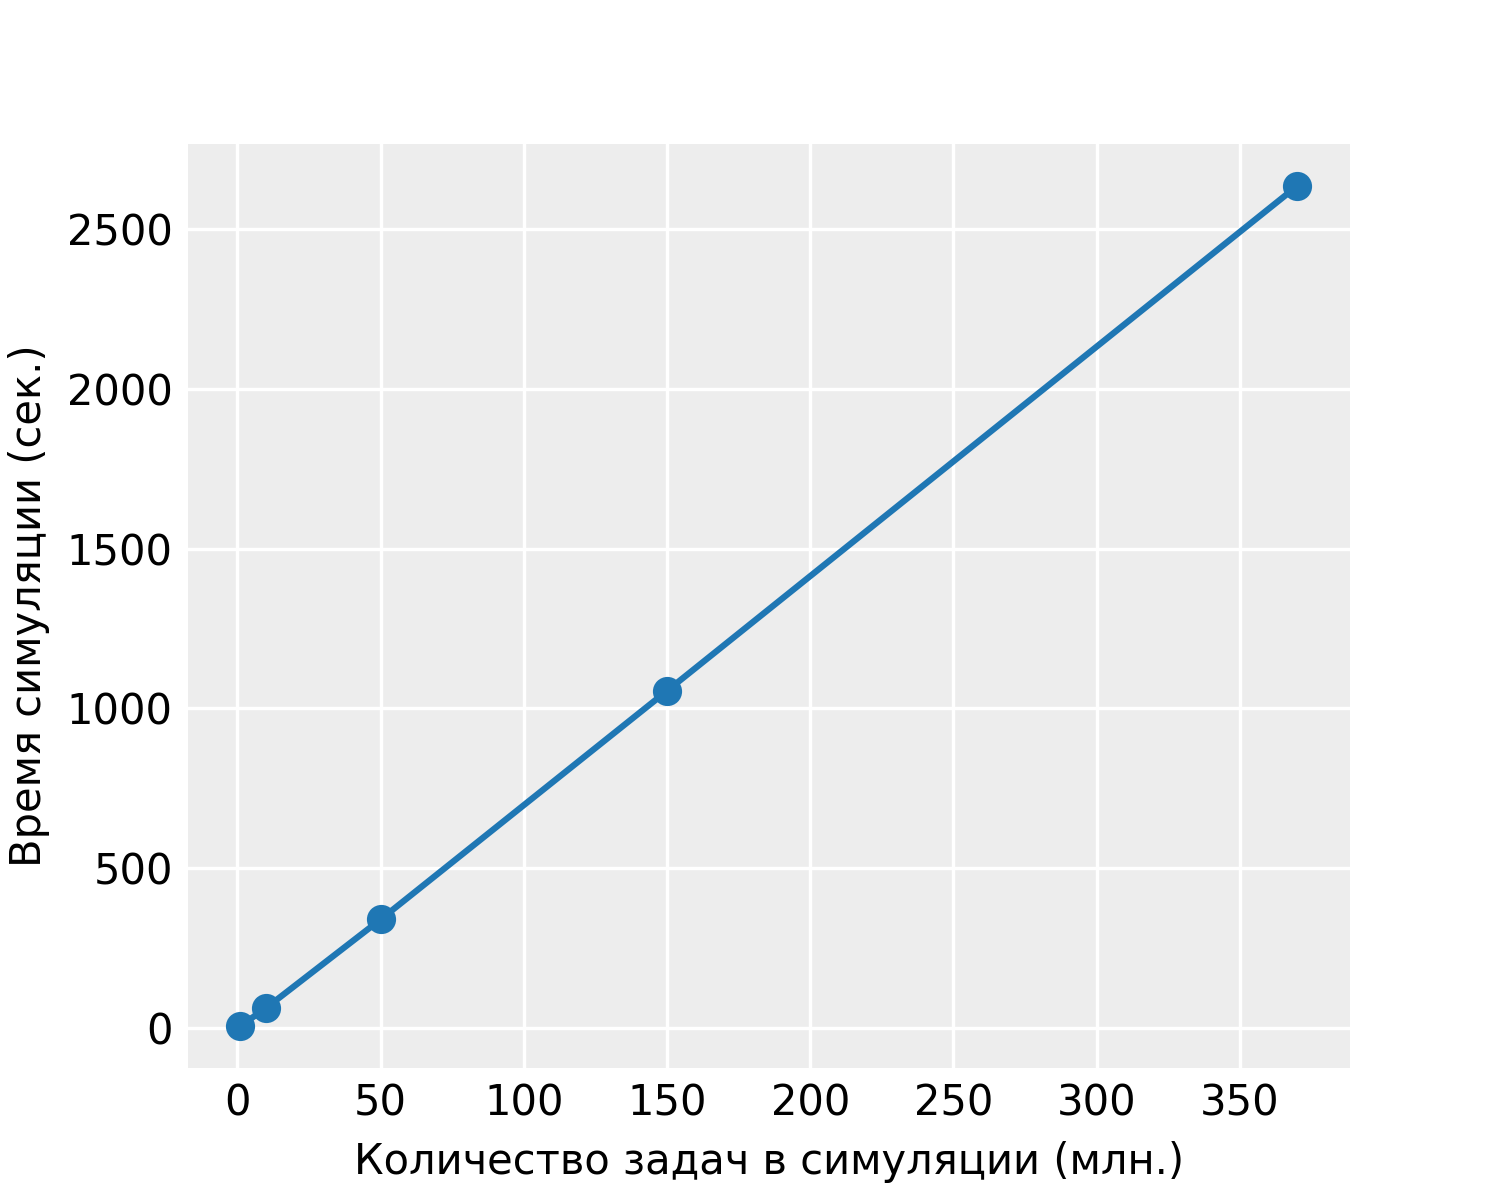
\includegraphics[width=\linewidth]{images/simulation_time}
		\caption*{Время работы симуляции в зависимости от количества задач}
	  \end{figure}
	\end{column} 
	\hspace{-1cm}
	\begin{column}{0.5\linewidth}
		\begin{itemize}
			\item На трейсе длиной 2.5 дня (350 млн задач, 25GB) время работы 45 минут
			\item Ускорение в 85 раз относительно реальной работы. 
			\item Необходимо сортировать трейс по времени.
			\item Без инкрементального чтения невозможно обработать трейс.
		\end{itemize}
	\end{column}
\end{columns}
\end{frame}

\section{Эксперименты: справедливость}

\subsection{\texttt{DRF} \& \texttt{Tetris} (Grandl и др., 2014).} 

\begin{frame}[fragile]
	\frametitle{\insertsection} 
	\framesubtitle{\insertsubsection}

	\begin{figure}[H]
		\centering
		\includegraphics<1>[width=0.8\linewidth]{images/tetris_pipeline_0} 
		\includegraphics<2>[width=0.8\linewidth]{images/tetris_pipeline_1} 
		\includegraphics<3>[width=0.8\linewidth]{images/tetris_pipeline_2} 
		\includegraphics<4>[width=0.8\linewidth]{images/tetris_pipeline_3} 
		\includegraphics<5>[width=0.8\linewidth]{images/tetris_pipeline_4} 
		\caption*{Работа \texttt{Tetris}. Коэффициент справедливости f.}
	\end{figure}


\end{frame}

\subsection{Набор серверов}

\begin{frame}[fragile]
	\frametitle{\insertsection} 
	\framesubtitle{\insertsubsection}

	\vspace{-0.5cm}
	
\begin{figure}[H]
    \centering 
    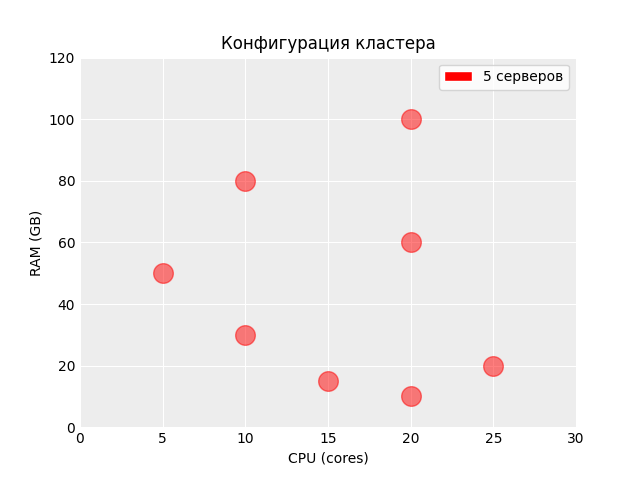
\includegraphics[width=0.8\linewidth]{images/hosts_distribution}
    \caption*{Распределение ресурсов на серверах кластера}
\end{figure}


\end{frame}

\subsection{Конфигурация пользователей}

\begin{frame}[fragile]
	\frametitle{\insertsection} 
	\framesubtitle{\insertsubsection}

	\vspace{0.5cm}
	
	\begin{table}[H]
		\footnotesize
		\centering
		\begin{tabular}{|c|c|c|c|c|c|}
			\hline
			\textbf{Имя} & \textbf{CPU} & \textbf{RAM} & \textbf{Кол-во задач} & \textbf{Duration Mean} & \textbf{Duration Dev} \\
			\hline
			user0 & 1 & 5 & 1500 & 250 & 40 \\
			\hline
			user1 & 1 & 10 & 800 & 400 & 40 \\
			\hline
			user2 & 1 & 15 & 800 & 300 & 30 \\
			\hline
			user3 & 2 & 5 & 1300 & 250 & 30 \\
			\hline
			user4 & 2 & 6 & 1200 & 250 & 30 \\
			\hline
			user5 & 2 & 7 & 800 & 300 & 40 \\
			\hline
			user6 & 5 & 4 & 1000 & 180 & 30 \\
			\hline
			user7 & 5 & 5 & 700 & 160 & 10 \\
			\hline
			user8 & 7 & 5 & 200 & 800 & 200 \\
			\hline
			user9 & 10 & 2 & 400 & 220 & 30 \\
			\hline
		\end{tabular}
		\caption*{Описание синтетической нагрузки на кластер}
	\end{table}

\end{frame}

\subsection{Результаты утилизации}

\begin{frame}[fragile]
	\frametitle{\insertsection} 
	\framesubtitle{\insertsubsection}

	\vspace{-0.5cm}
	
	\begin{columns}
		\begin{column}{0.6\linewidth}
			\begin{figure}[H]
				\centering 
					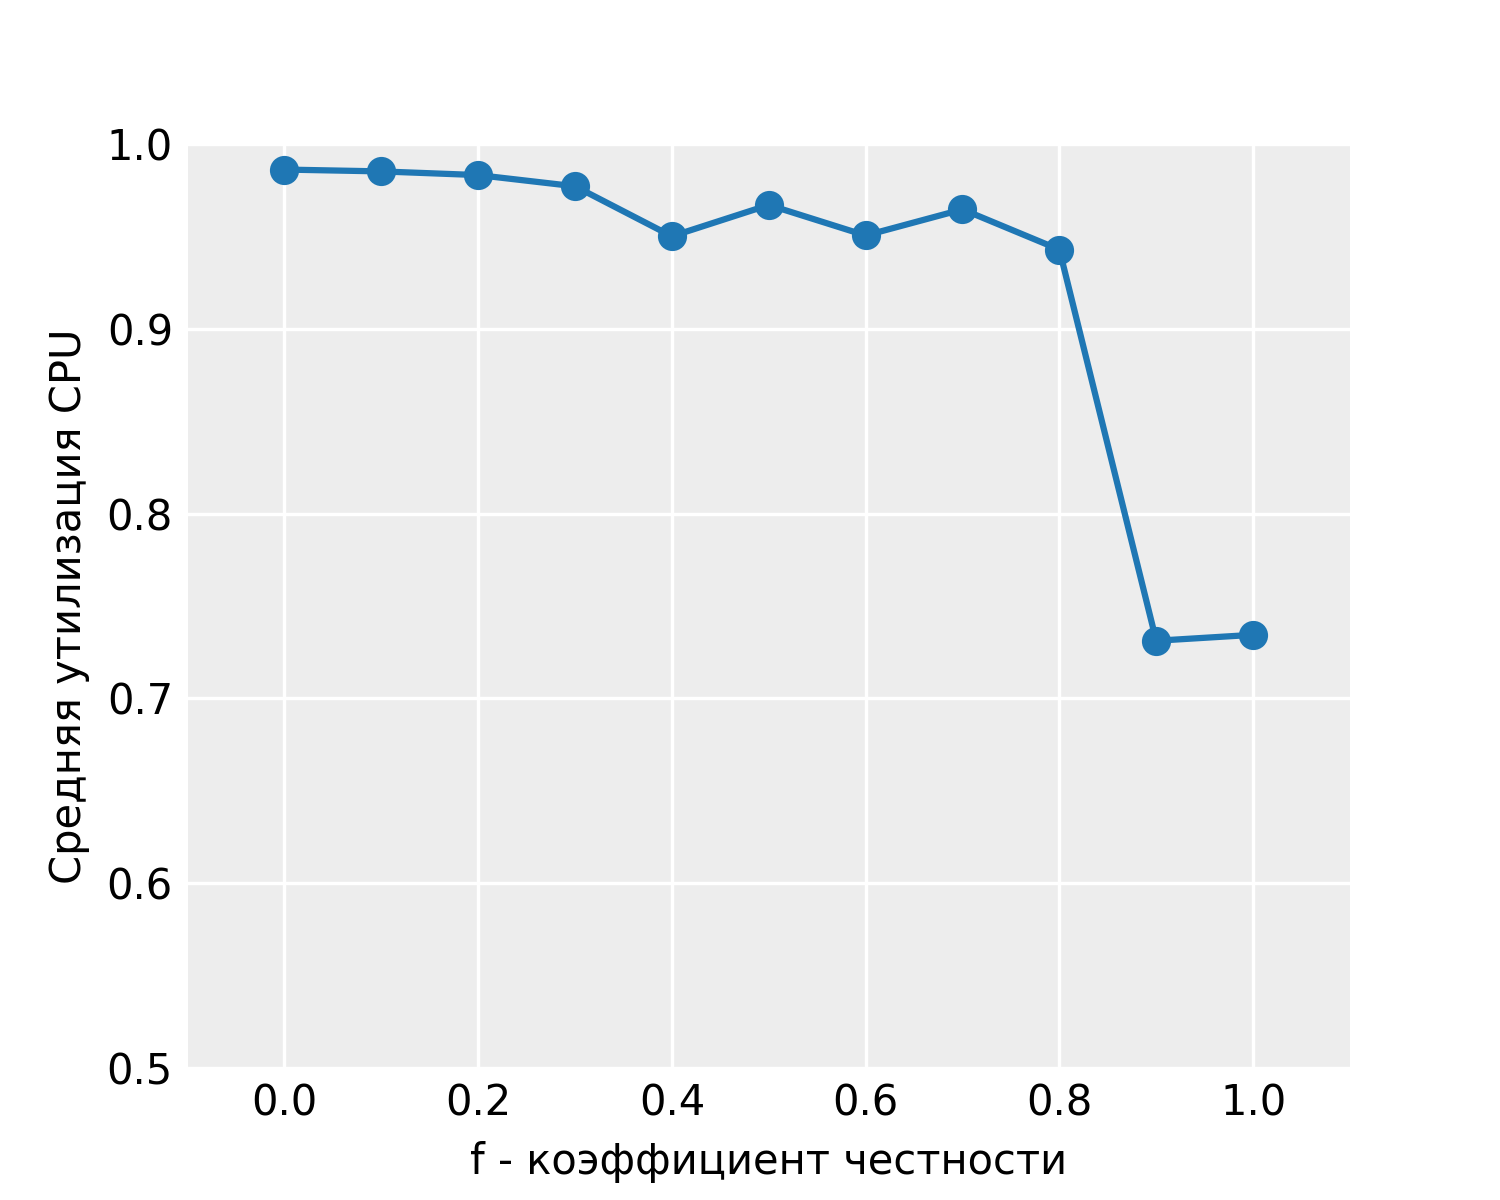
\includegraphics[width=\linewidth]{images/cpu_utilization}
					\caption*{Утилизация CPU при разных $f$}
				\end{figure}
		\end{column}
		\hspace{-0.5cm}
		\begin{column}{0.6\linewidth}
			\begin{figure}[H]
				\centering 
					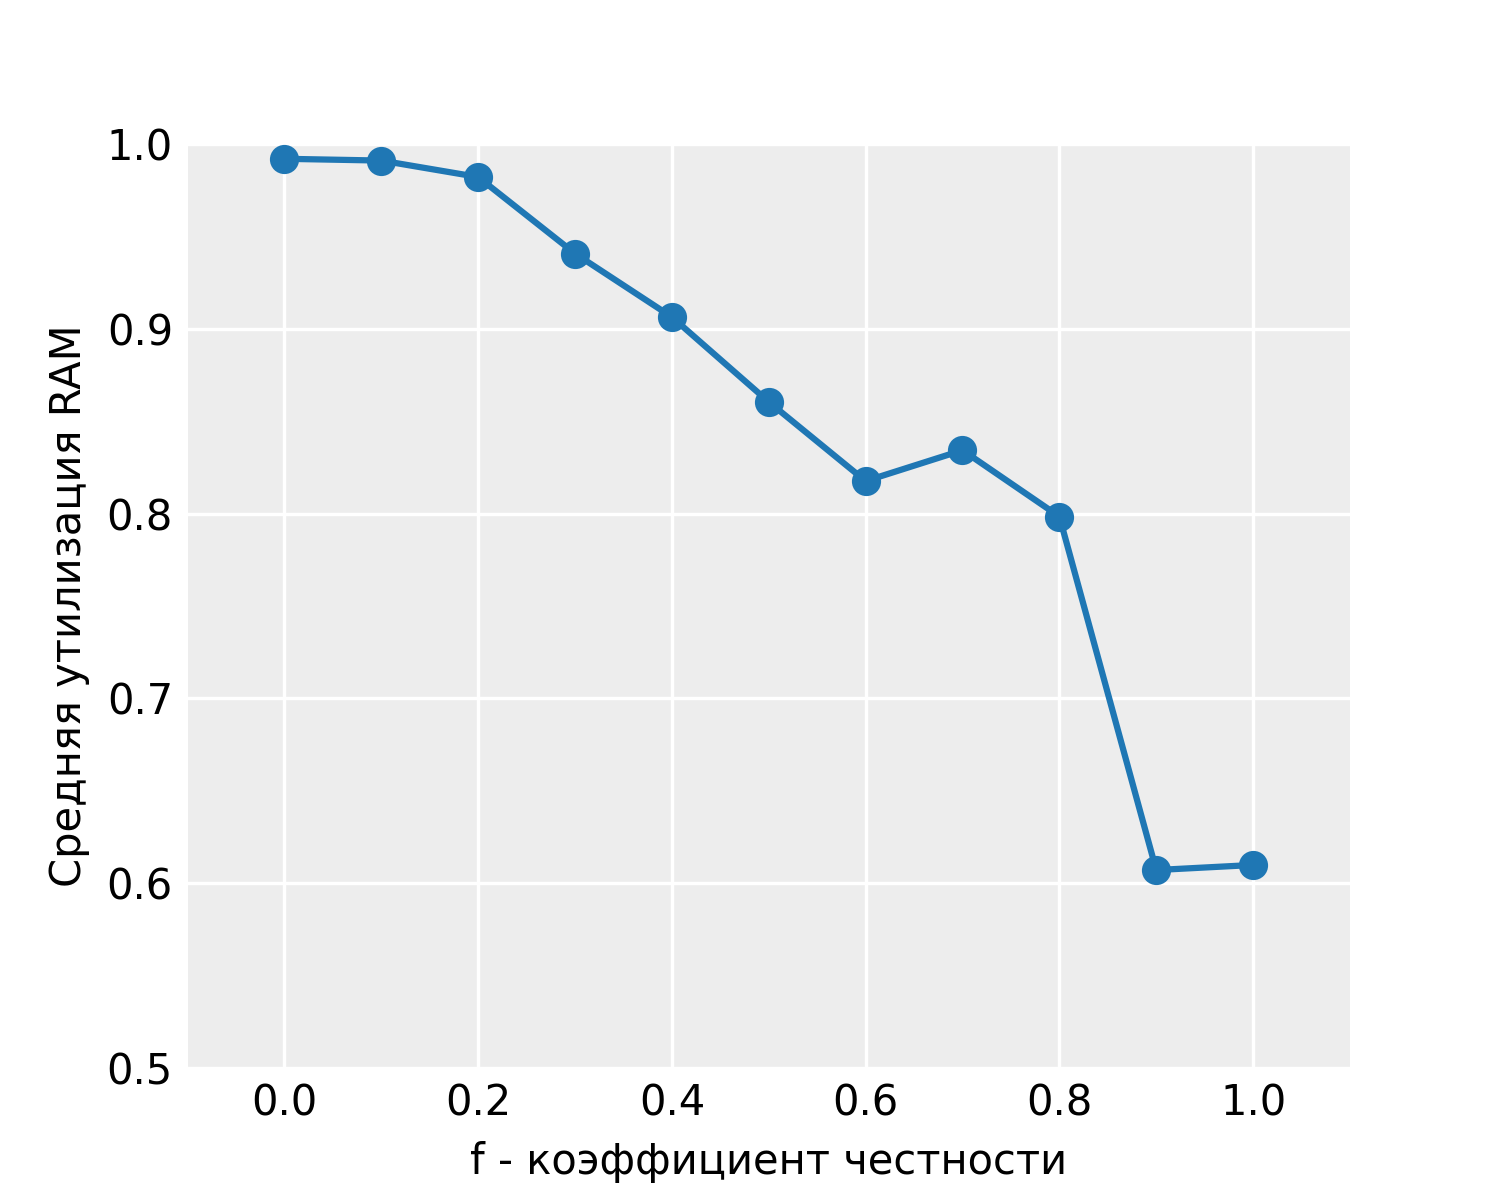
\includegraphics[width=\linewidth]{images/memory_utilization}
					\caption*{Утилизация RAM при разных $f$}
				\end{figure}
		\end{column}
	\end{columns}

	
\end{frame}




\subsection{Результаты справедливости}

\begin{frame}[fragile]
	\frametitle{\insertsection} 
	\framesubtitle{\insertsubsection}

	\vspace{-0.5cm}
	
	\begin{columns}
		\begin{column}{0.65\linewidth}
			\begin{figure}[H]
				\centering 
					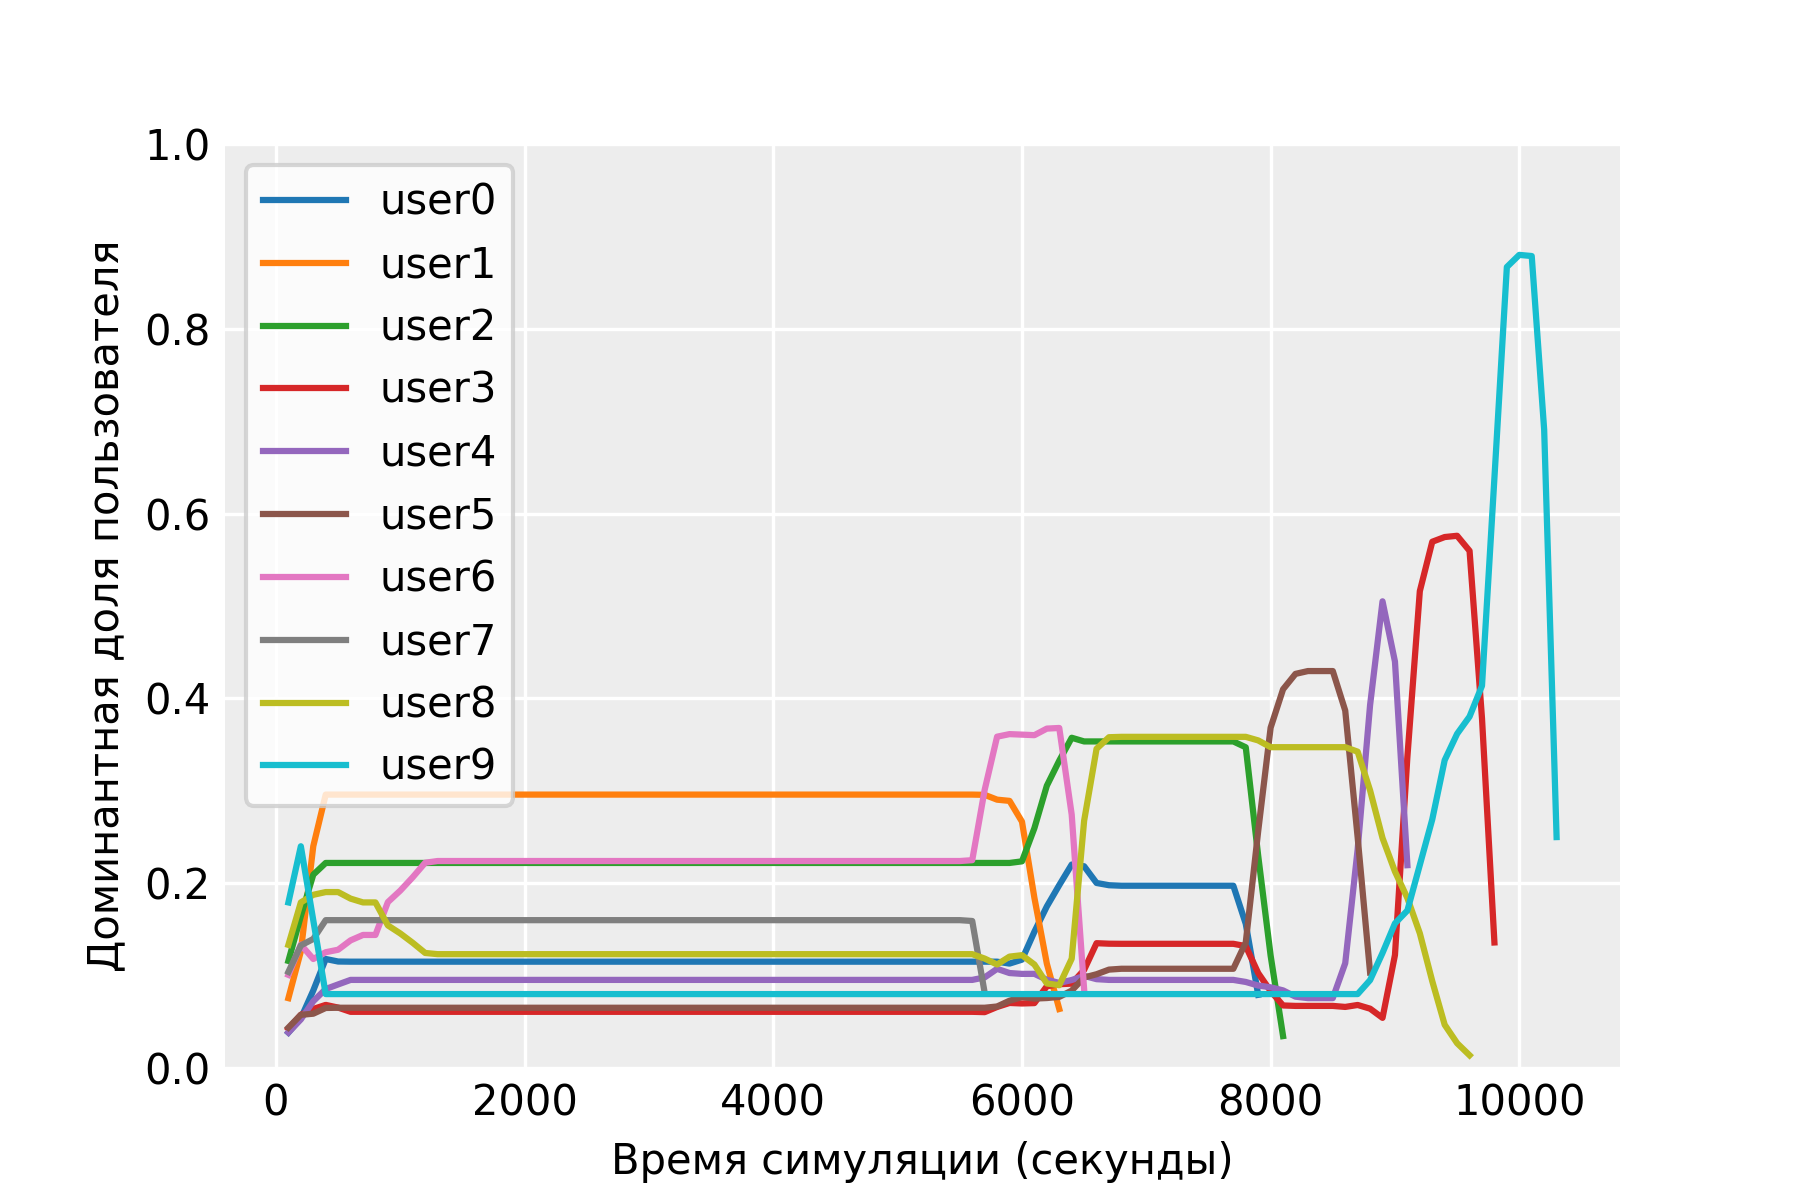
\includegraphics[width=\linewidth]{images/fair_share_0}
					\caption*{$f = 0$}
				\end{figure}
		\end{column}
		\hspace{-1cm}
		\begin{column}{0.65\linewidth}
			\begin{figure}[H]
				\centering 
					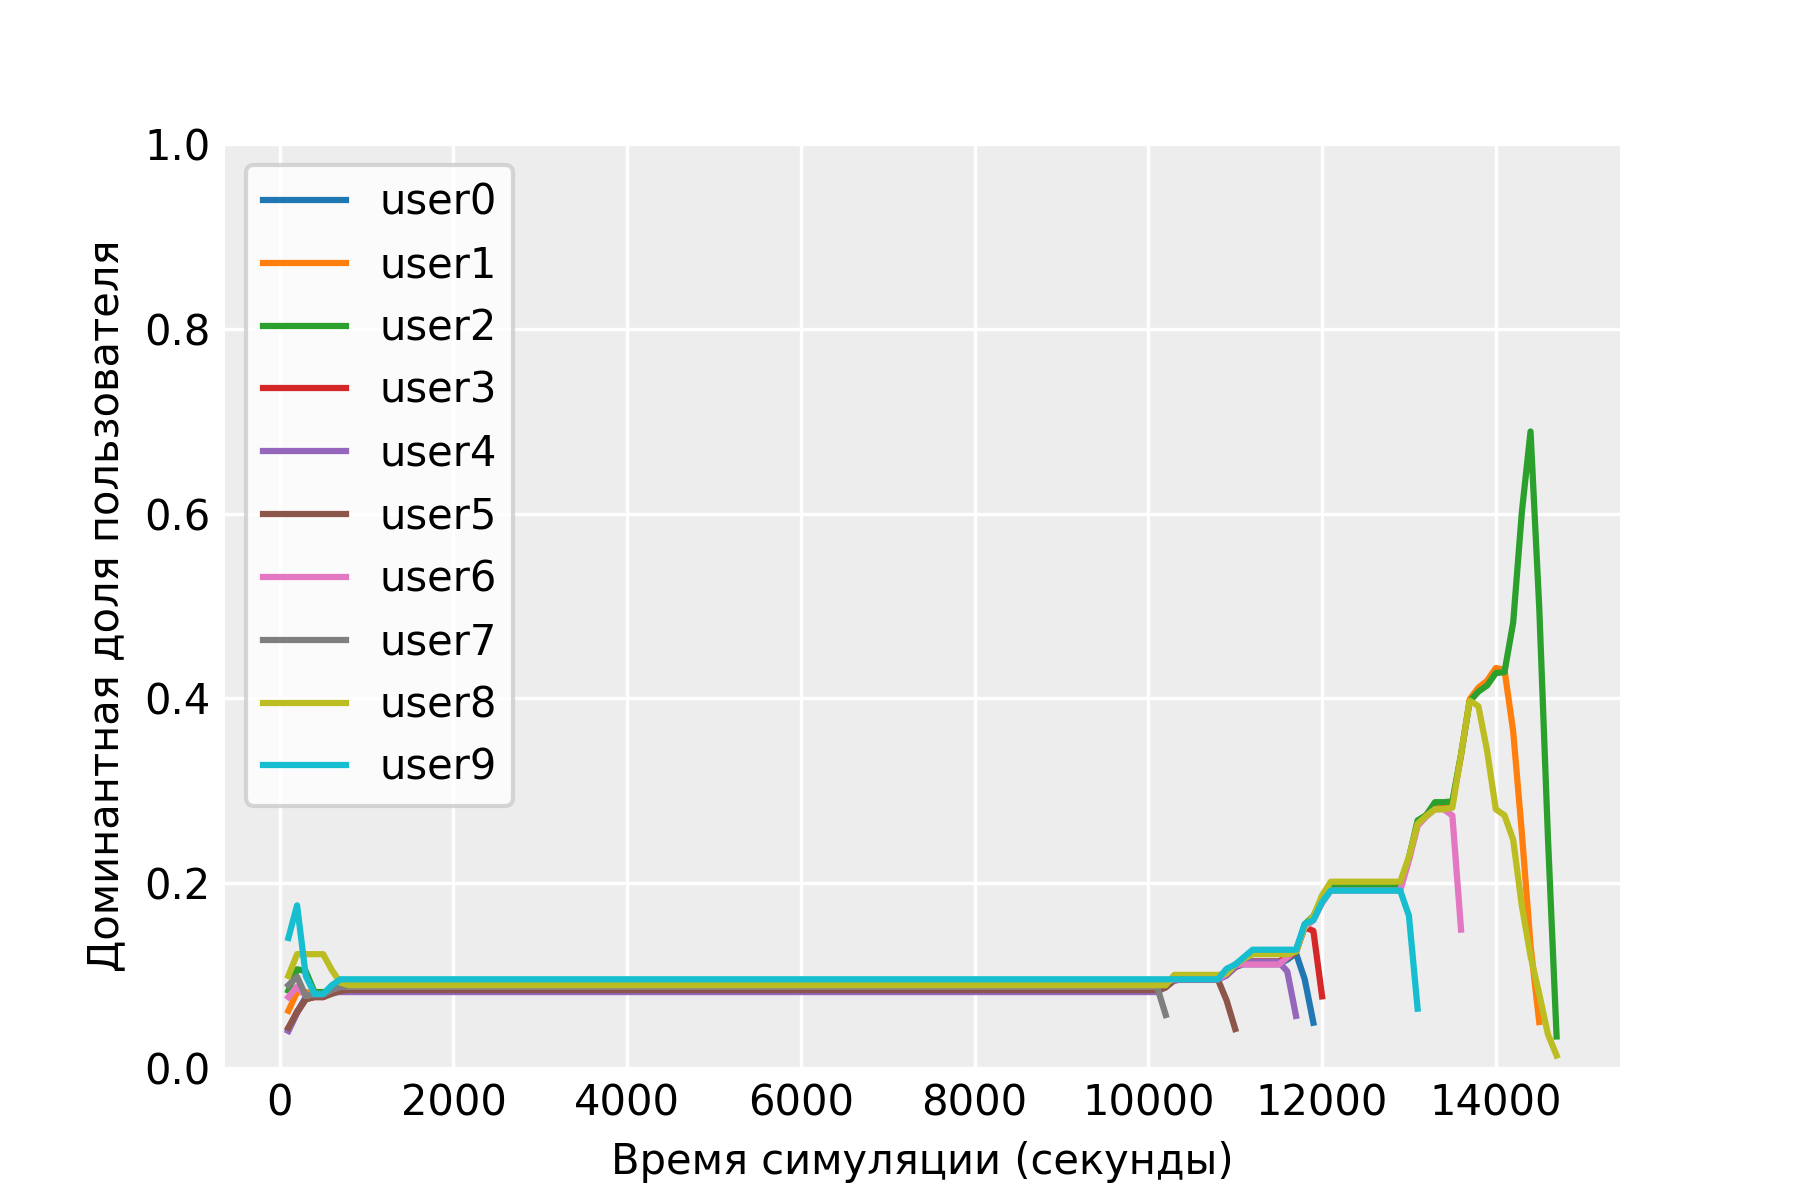
\includegraphics[width=\linewidth]{images/fair_share_1}
					\caption*{$f = 1$}
				\end{figure}
		\end{column}
	\end{columns}

	
\end{frame}


\begin{frame}[fragile]
	\frametitle{\insertsection} 
	\framesubtitle{\insertsubsection}

	\vspace{-0.5cm}
	
	\begin{columns}
		\begin{column}{0.65\linewidth}
			\begin{figure}[H]
				\centering 
					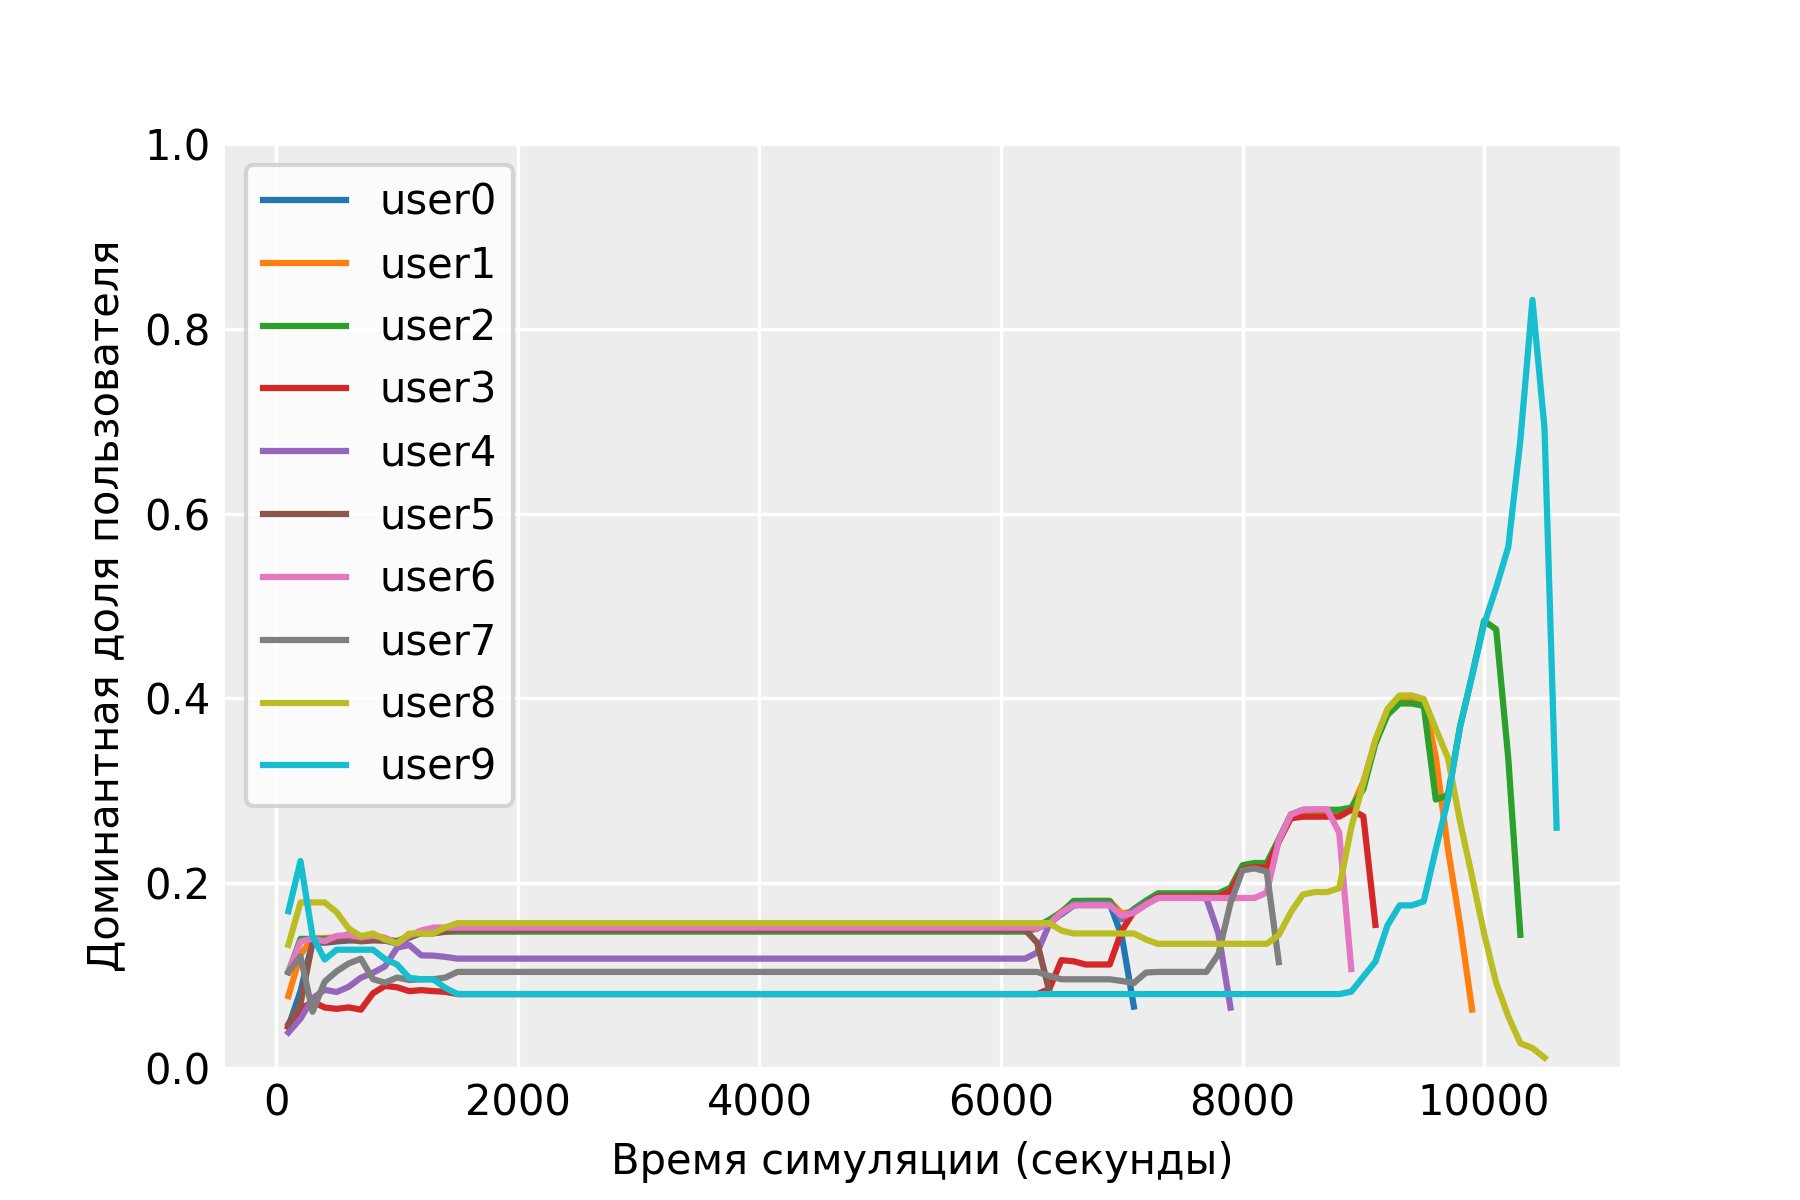
\includegraphics[width=\linewidth]{images/fair_share_05}
					\caption*{$f = 0.5$}
				\end{figure}
		\end{column}
		\hspace{-1cm}
		\begin{column}{0.65\linewidth}
			\begin{figure}[H]
				\centering 
					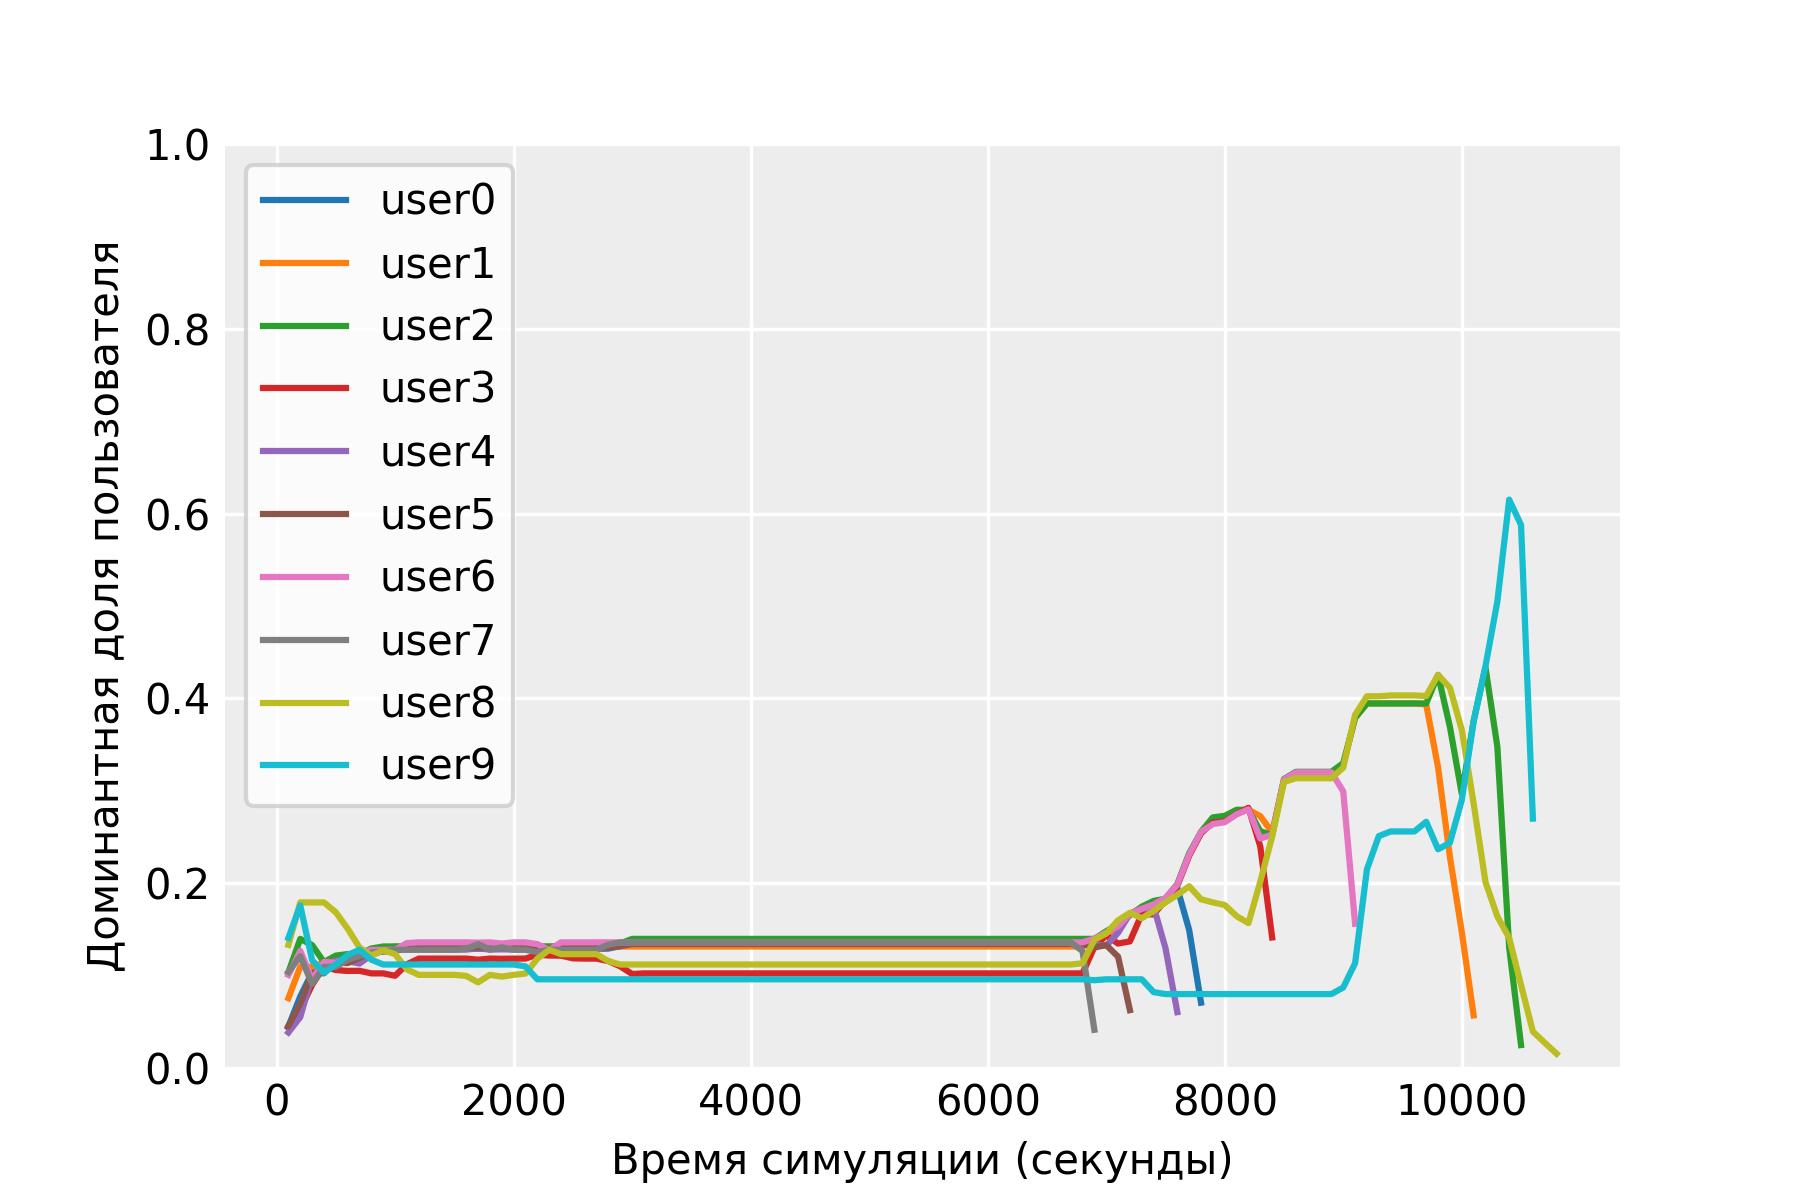
\includegraphics[width=\linewidth]{images/fair_share_06}
					\caption*{$f = 0.6$}
				\end{figure}
		\end{column}
	\end{columns}

	\alt<2->{
		\textbf{Вывод:} $f = 0.6$ -- оптимальный параметр честности для такой конфигурации кластера и задач пользователей. 
	}{}

	
\end{frame}


	\section{Заключение}

	\begin{frame}[fragile]
		\frametitle{\insertsection} 
		\framesubtitle{\insertsubsection}
		\small
		\vspace{-0.5cm}
		\hspace*{-0.5cm}
		\begin{minipage}{1.1\linewidth}
			{\centering
		\begin{itemize}
			\item<1->[\ding{51}] Реализовать эффективный симулятор вычислительного кластера.
			\item<2->[\ding{51}] Поддержать несколько моделей рабочей нагрузки и планирования заданий.
			\item<3->[\ding{51}] Поддержать чтение трейсов нагрузки компаний (Google, Alibaba).
			\item<4->[\ding{51}] Поддержать адаптивный сбор статистики для анализа результатов (нагрузка на кластер, честность, статистика очереди)
			\item<5->[\ding{51}] Реализовать несколько популярных алгоритмов (FCFS, DRF, Tetris).
			\item<6->[\ding{51}] Доработать реализацию асинхронного ядра \texttt{dslab-core} и ускорить его работу в 2 раза.
			% \item<7->[\ding{51}] Улучшить модель мгновенной честной доли и добавить в нее возможность отмены активностей.
		\end{itemize}
			}
			\vspace{0.2cm}
			\alt<7->{
		\textbf{Главное достижение:} предоставить возможность описывать рабочую нагрузку в виде асинхронных примитивов языка \texttt{Rust}.
			}{}
			
	\end{minipage}

	\end{frame}

	% \section{Основные источники}
	% \begin{frame}
	% 	\frametitle{\insertsection} 
	% 	\framesubtitle{\insertsubsection}
	% 	\vspace{1cm}	
	% 	\begin{enumerate}
	% 		\item The standard workload format specification. \url{https://www.cs.huji.ac.il/labs/parallel/workload/swf.html}
	% 		\item Dslab repository. \url{https://github.com/osukhoroslov/dslab}
	% 		\item BatSim docs. \url{https://batsim.readthedocs.io/en/latest/}
	% 	\end{enumerate}
	% 	% \printbibliography
	% \end{frame}

	\section{Приложения}
	
	\begin{frame}{\textbf{Вопросы}}
	
		\begin{enumerate}
			% \item \hyperlink{batsim-compare}{\nameref{batsim-compare}}
			\item \hyperlink{drf-fairness}{\nameref{drf-fairness}}
			\item Профили нагрузки по умолчанию 
			\item Выходные данные и monitoring 
			\item Ускорение async-dslab-core в 2 раза 
			\item \hyperlink{dsmodeling}{\nameref{dsmodeling}} 
		\end{enumerate}
	\end{frame}

	\subsection{\texttt{Сравнение с симулятором \texttt{BatSim}}}\label{batsim-compare}

	\begin{frame}[fragile]
		\frametitle{\insertsection} 
		\framesubtitle{\insertsubsection}
		\vspace{1cm}	
		\begin{itemize}
			\item Разработан на базе фреймворка \texttt{SimGrid}.
			\item Поддерживает \texttt{SWF} и пользовательские профили нагрузки через JSON-файл.
			\item Алгоритмы планирования подключаются к симулятору через IPC (inter-process-communication).
		\end{itemize}
		\end{frame}


	\subsection{\texttt{Профиль нагрузки в BatSim}}
	\begin{frame}[fragile]
		\frametitle{\insertsection} 
		\framesubtitle{\insertsubsection}
		\begin{figure}
			\scriptsize
		\begin{jsoncode}
"jobs": [
  {"id": "job1",  ...  "res": 4, "profile": "sequence"},
],

"profiles": {
  "homogeneous": {
    "type": "parallel_homogeneous",
    "cpu": 10e6,
    "com": 1e6
  },
  "sequence": {
    "type": "composed",
    "repeat" : 4,
    "seq": ["simple","homogeneous","simple"]
  },
}
		\end{jsoncode}
	\end{figure}
	\end{frame}



\subsection{Алгоритмы справедливости. \texttt{DRF} \& \texttt{Tetris}}\label{drf-fairness}


\begin{frame}[fragile]
	\frametitle{\insertsection} 
	\framesubtitle{\insertsubsection}

	\begin{columns}[t] 
		\begin{column}{0.7\linewidth}
			\begin{figure}[H]
			\centering 
			\includegraphics<1>[width=\linewidth]{images/drf_1}
			\includegraphics<2->[width=\linewidth]{images/drf_2}
			\caption*{Потребление ресурсов пользователями}
			\end{figure}			
		\end{column}
		\hspace{-1cm}
		\begin{column}{0.35\linewidth}
			\alt<2->{
				\vspace{0.6cm}

			Dominant shares:
			\begin{itemize}
				\item USER1 = $1/10$
				\item USER2 = $1/5$
				\item<3-> USER1 первый получит ресурсы
			\end{itemize}
			}{}
		\end{column}
	\end{columns}

\end{frame}


\begin{frame}
\frametitle{\insertsection}
\framesubtitle{\insertsubsection}

Метрика <<упаковки>>: $H_{angle} = 1 - \cos(\measuredangle(Task_{res}, Server_{res}) )$

\alt<2->{
\begin{figure}
	\centering 
	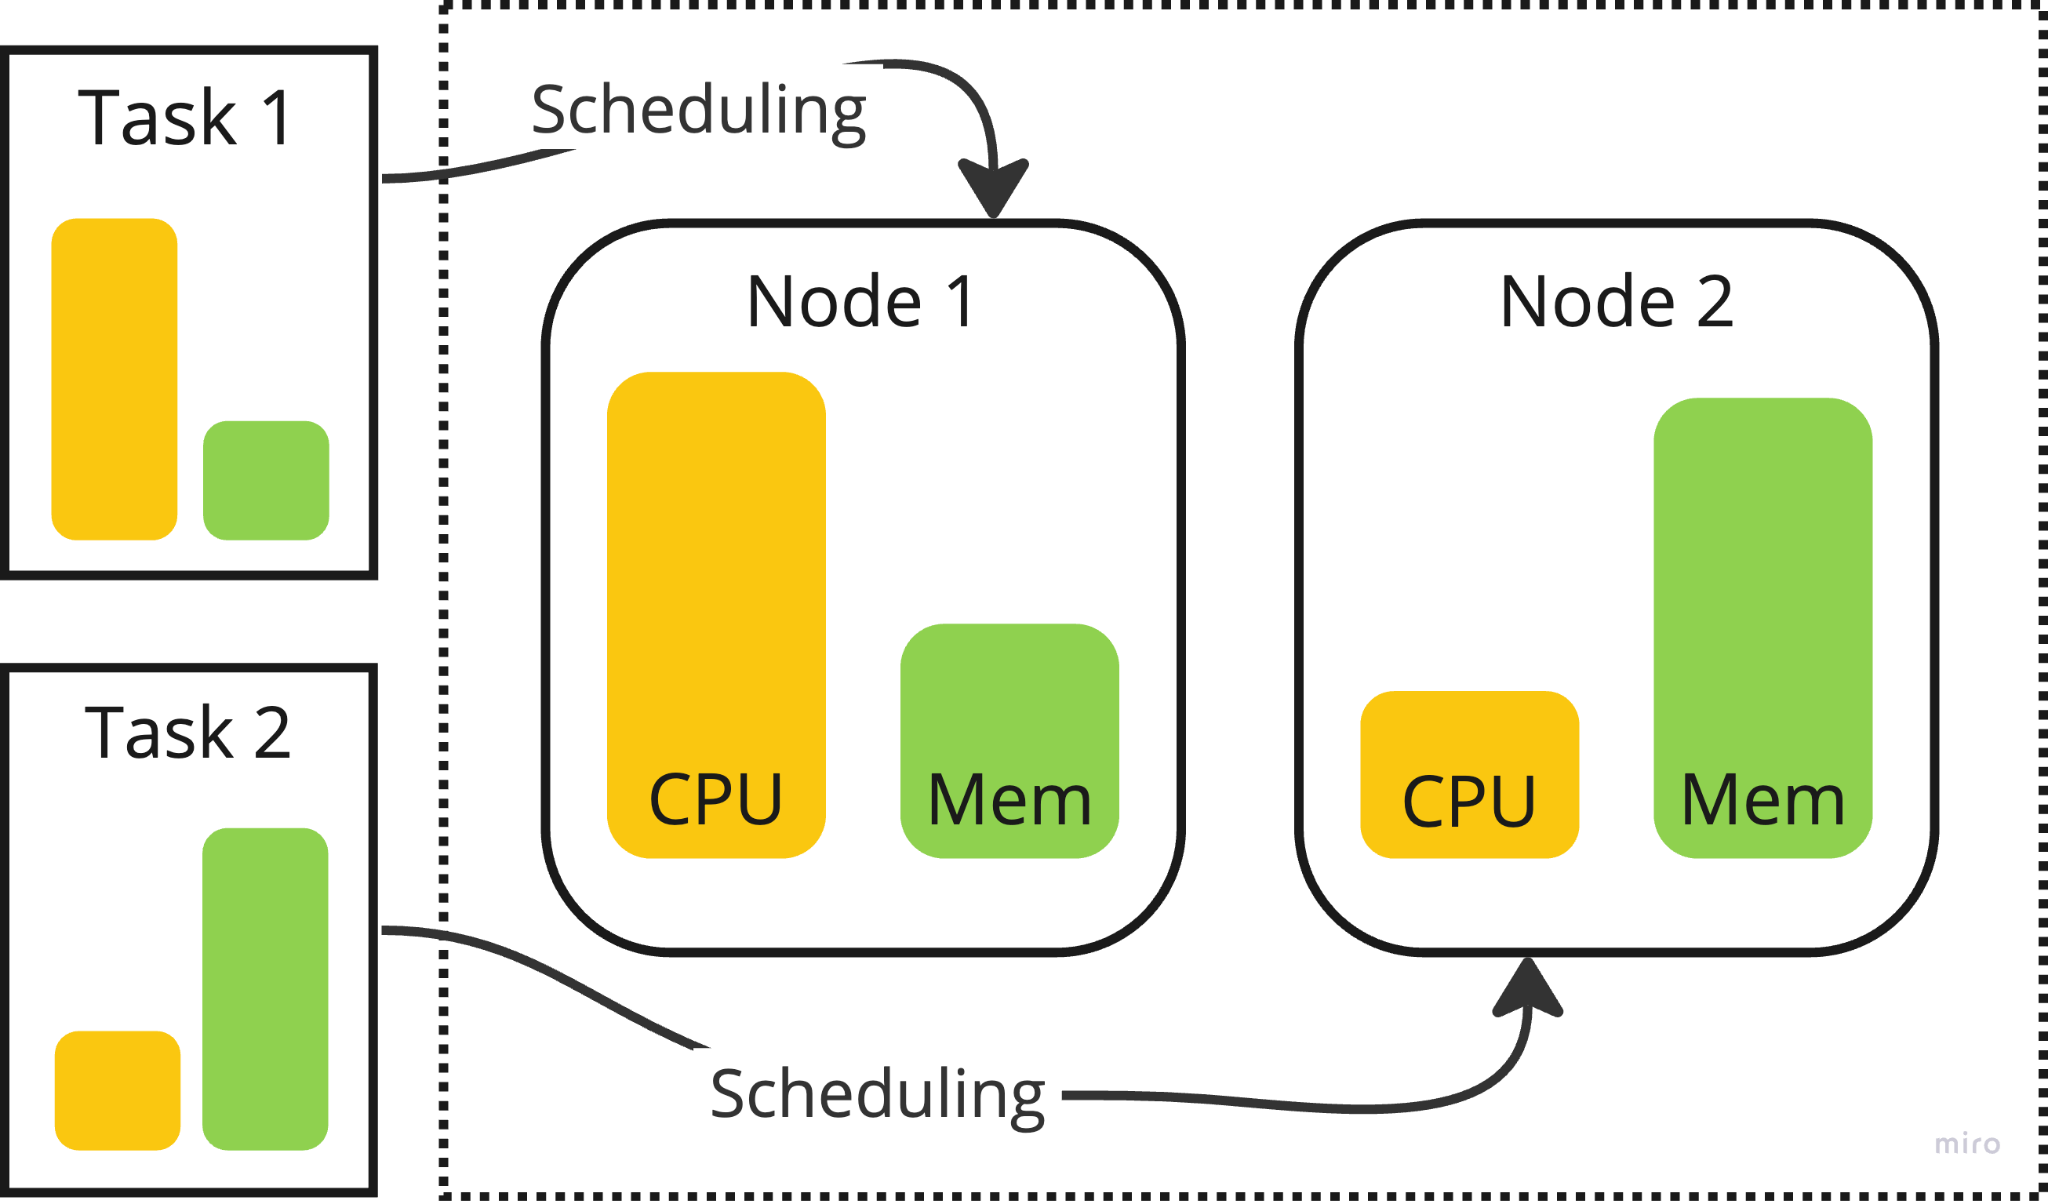
\includegraphics[width=0.8\linewidth]{images/tetris_match}
	\caption*{Пример работы алгоритма \texttt{Tetris}}
\end{figure}
}{}

\end{frame}

\subsection{Как устроено дискретно-событийное моделирование}\label{dsmodeling}
\begin{frame}
    \frametitle{\insertsection} 
	\framesubtitle{\insertsubsection}

	\begin{figure}
		\centering
		{
		\includegraphics<1>[width=\linewidth]{images/event_pipeline_0}
		\includegraphics<2>[width=\linewidth]{images/event_pipeline_1}
		\includegraphics<3>[width=\linewidth]{images/event_pipeline_2}
		\includegraphics<4>[width=\linewidth]{images/event_pipeline_3}
		\includegraphics<5>[width=\linewidth]{images/event_pipeline_4}
		\includegraphics<6>[width=\linewidth]{images/event_pipeline_5}
		\includegraphics<7>[width=\linewidth]{images/event_pipeline_6}
		\includegraphics<8>[width=\linewidth]{images/event_pipeline_7}
		\includegraphics<9>[width=\linewidth]{images/event_pipeline_8}
		\includegraphics<10>[width=\linewidth]{images/event_pipeline_9}
		}
		\caption*{Исполнение симуляции}
	\end{figure}
    \end{frame}


\end{document}